% Preamble
\documentclass[preprint,10pt]{elsarticle}
\linespread{1.25}

% (preamble packages as shared)
\usepackage[dvipsnames]{xcolor}
\bibliographystyle{chicago}
\usepackage{natbib}
\setcitestyle{authoryear}
\usepackage{graphicx}
\usepackage{makecell}  
\usepackage{amsmath,amsfonts,amssymb,bbm}
\usepackage{threeparttable,longtable,threeparttablex,booktabs}
\usepackage{lscape,rotfloat,subcaption,placeins}
\usepackage{geometry,setspace}
\usepackage{lineno}
\usepackage{tikz}
\usetikzlibrary{arrows.meta,positioning,fit,backgrounds,calc}
\usepackage[colorlinks,citecolor=blue,urlcolor=blue]{hyperref}
\usepackage[utf8]{inputenc}
\usepackage[T1]{fontenc}
\usepackage[ruled,vlined,linesnumbered]{algorithm2e}
\DontPrintSemicolon
\SetKwComment{tcp}{$\triangleright$ }{}           % right-margin comments
\SetAlgoNlRelativeSize{-1}                         % smaller line numbers
\setlength{\algomargin}{1.2em}                     % tighter left margin
\SetInd{0.4em}{0.8em}                              % tighter indent
\setlength{\interspacetitleruled}{2pt}             % compact title spacing
\setlength{\algotitleheightrule}{0.4pt}
\setlength{\algoheightrule}{0.4pt}
\setcounter{secnumdepth}{4}
\setcounter{tocdepth}{4}
\geometry{footskip=120pt}
\captionsetup[table]{position=below}

% Journal and author info
\journal{Global Finance Journal}
\AtBeginDocument{
  \renewcommand{\sectionautorefname}{Section}
  \renewcommand{\subsectionautorefname}{Subsection}
}

\begin{document}
\begin{frontmatter}

\title{State-Dependent Pricing in FinTech Credit: Evidence from P2P Lending}
\author[aff1,aff2,cor1]{Lennart John Baals}
\author[aff1]{Jörg Osterrieder}
\author[aff2]{Ali Hirsa}
\address[aff1]{Department of Industrial Engineering and Business Information Systems, University of Twente, Building 10: Ravelijn, Drienerlolaan 5, Enschede, The Netherlands}
\address[aff2]{Department of Industrial Engineering and Operations Research, Columbia University, 500 W. 120th Street, New York, NY 10027, USA}
\cortext[cor1]{Corresponding author: l.j.baals@utwente.nl}

\begin{abstract}
This paper develops a transparent framework to detect state-dependent loan pricing in peer‑to‑peer (P2P) lending. A rolling robust principal‑component analysis (R2‑PCA) is utilised to compresses 774 macroeconomic indicators, yielding eight factors with the highest average absolute loadings. These indicators are subsequently fed into a parsimonious Hidden Markov Model (HMM) to distinguish between accommodative and restrictive regime phases. Through an explainability layer based on cross‑validated decision trees, posterior regime probabilities are converted into threshold rules for the observed indicators, notably labor‑market stress and short‑term funding spreads. Subsequent regression analysis of credit spreads derived from a sample of 93{,}135 LendingClub loans restricted to an underwriting regime between 2007 and 2012 show a general risk‑premium widening in restrictive months that is increasing in borrower risk and stronger at longer maturities. Credit spreads increase by about 60 to 210 basis points (bp) from Grade~A to Grade~G, and by 59~bp for 36‑month versus 133~bp for 60‑month contracts after controlling for borrower covariates and clustering by issuance month. The findings document regime‑dependent pricing with pronounced grade and tenor gradients in algorithmically intermediated credit, with implications for platform pricing and risk management in fintech credit markets.
\end{abstract}


\begin{keyword}
P2P lending \sep Macro–credit regimes \sep Regime switching \sep Hidden Markov models \sep Rolling PCA \sep Credit spreads
\end{keyword}

\end{frontmatter}


\newpage
%========== MAIN BODY ==========
%======================================================
\section{Introduction}
%======================================================

Over the past decade, platform intermediation and automated underwriting have reshaped lending markets, transforming how financial services are produced and delivered \citep{serfes_fintech_2025,berg_fintech_2022}. Among the most prominent financial technology (FinTech) applications is \emph{peer‑to‑peer} (P2P) lending, a platform‑based lending channel that matches individual lenders and borrowers directly, bypassing balance‑sheet intermediation \citep{philippon_fintech_2016,balyuk_fintech_2023}. As loan originations occur online with fewer disclosure requirements, P2P loans offer borrowers with limited collateral a new source of funding, while promising lenders adequate compensation for elevated credit risk. This commonly positions marketplace lending as a substitute for traditional banking services \citep{tang_peer--peer_2019}. As a result, global P2P volumes have exceeded~USD~90~billion in 2023, and the segment is found to continuously grow.\footnote{Data from the Cambridge \emph{Alternative Finance Benchmarking Report}, 2024.} Loan pricing in P2P lending, however, may not be immune to macro‑financial forces and the effect of changes in macro-economic conditions on credit spreads of P2P loans have rarely been studied so far. \cite{a_basha_online_2021} reviewed the P2P lending literature and conclude that most scholarly work is heavily skewed towards the impact of microeconomic factors on P2P lending, leaving the effect of macroeconomic factors unexplored. 

However, the impact of macro economic forces on traditional consumer lending markets is well documented. Credit prices are commonly found to move with macro economic conditions. In economic downturns, as household financial positions deteriorate, lenders tend to raise required premia and tighten credit supply. This pattern is specifically observable in consumer and mortgage credit, where risk-based pricing and the dispersion of rates increase as borrower risk rises and collateral values fall \citep{edelberg_risk-based_2006,adams_liquidity_2009,mian_house_2011}. Monetary policy and funding conditions are also found to indirectly shape loan pricing, with shifts in policy rates affecting the credit supply, loan quality of incoming borrowers, and risk taking by banks \citep{jimenez_hazardous_2014,heider_life_2019,bernanke_inside_1995}. Marketplace lending may be subject to the same forces even though the intermediation technology differs. Platform design determines how information is reflected in the interest rates and how investor demand is serviced \citep{vallee_marketplace_2019,wei_market_2016}, which means macro shocks can alter both the level of interest premia and their sensitivity to borrower risk.

Thus far, only a few studies have attempted to link monetary policy, unemployment gaps, inflation hikes, and market volatility to credit risk and primary-market pricing on leading U.S.\ and European P2P platforms \citep{foo_discovering_2023,baumohl_macroeconomic_2024,nigmonov_macroeconomic_2022,avgeri_factors_2024}. A common attribute among all of them is that methodological approaches have primarily focused on a small set of preselected macro-economic factors and typically adopt a static temporal view. This perspective could be expanded, as credit cycles are more often characterized by state-dependent dynamics \citep{gambacorta_impact_2020}. To our knowledge, no prior work has systematically investigated the influence of macroeconomic factors and state-dependence in P2P loan pricing, even though dynamic structural models are standard in equity and corporate-bond markets where changes in means, volatilities, and loadings are observed \citep{ang_regime_2002,ang_regime_2012,davies_credit_2004,davies_credit_2008,alexander_regime_2008,maalaoui_chun_credit_2014}. Extending these tools to P2P lending requires careful consideration as platform rules and grade cutoffs can shift over time and the macro panels are high dimensional, so identifying regimes and linking them to primary-market coupons demands a holistic data driven approach.

Therefore, we introduce a modeling process that considers the state-dependent nature of credit markets, where macroeconomic shocks can have opposite effects depending on the prevailing regimes, a phenomenon well-documented in traditional banking \citep{bernanke_inside_1995} but unexplored in P2P markets. First, we employ a keyword centric feature reduction approach followed by a rolling-robust-principal‑component algorithm (R2-PCA) of \citet{hirsa_robust_2023} to compress 774~series from the Federal Reserve Economic Database (FRED) into a principle component (PC) space that adapts to shifting covariance structures.\footnote{Further details on the explicit keyword terminology used can be found in Table~\ref{tab:keyword_pipeline_dense}.} Second, we feed the leading 8 macro factor scores into a parsimonious rolling-robust regime detection (R2-RD) model \citep{hirsa_robust_2024} that builds on a Hidden Markov architecture to decode \emph{accommodative} and \emph{restrictive} macro‑credit regimes. Third, we establish an explainability step in form of a cross‑validated surrogate decision tree that translates the latent states into a hierarchy of threshold rules based on the observable macro indicators. Our empirical analysis covers June~2007–March~2025 at the macro level. For loan‑level pricing tests, we restrict the sample to a pre‑2013 underwriting regime to ensure stable credit grade definitions, yielding \(93{,}135\) LendingClub loans issued between June~2007 and December~2012.\footnote{See \autoref{subsec:loan_data} for sample construction.} 

Our analysis empirically yields an operational regime signal that is found to significantly price primary-market P2P loans. The restrictive macro–credit regime translates into higher coupon spreads across all grades and maturities. Credit spreads increase with gradients by risk and term (\(\approx +60\)~bp for Grade A up to \(\approx +210\)~bp for Grade G; \(\approx +59\)~bp for 36-month vs. \(\approx +133\)~bp for 60-month loans). Through the integrated study design we transparently trace the distressed regime signal and convert the latent state into simple threshold rules for the observed indicators. To our knowledge, this is the first study to document state-dependent loan pricing in P2P markets, and to deliver an implementable set of rules for considering macro economic factors in the rate-setting process of P2P loans. Hence, this study contributes to the current literature on macro determinants in P2P credit pricing in the following: (\emph{i}) We develop a transparent approach to produce a time-consistent regime signal and testable thresholds in observable macro indicators related to P2P marketplace lending that are determined by the data rather then assumed as in previous studies (see \cite{foo_discovering_2023}, \cite{nigmonov_macroeconomic_2022}, \cite{baumohl_macroeconomic_2024}). (\emph{ii}) In building on the contribution of \cite{davies_credit_2004, davies_credit_2008} who find that incorporating volatility regimes adds to the explanatory power of credit-spread determinants (see also \cite{alexander_regime_2008, maalaoui_chun_credit_2014}), we extend this insight to P2P lending. Empirically, we showcase that regime‑dependent pricing in P2P loans significantly manifests as a uniform risk‑premium widening that is monotone in borrower risk and stronger at longer maturities. (\emph{iii}) By translating the latent regime states into four simple, sample-invariant threshold rules on labour- and short-term funding stress, we derive a decision basis that investors can utilize for macro economic pricing in P2P credit. 

The remainder of this study is organized as follows. Section~\ref{sec:lit_review} reviews the literature on P2P pricing and macro-credit regimes and states the hypotheses. Section~\ref{sec:data} describes the macro-financial panel and the loan-level sample and summarizes the preprocessing. Section~\ref{sec:method_frame} outlines the methodological framework that builds the data-driven regime signal, explains the decoded states with simple decision rules, and sets up the loan-level pricing tests. Section~\ref{sec:results} presents the empirical results together with robustness checks and discusses their economic significance. Section~\ref{sec:conclusion} concludes and highlights directions for future research.


\section{Literature Review and Hypothesis}
\label{sec:lit_review}

\subsection{P2P Loan Pricing and the Influence of Macro Determinants}
\label{subsec:macro_determinant}

The literature on P2P loan pricing decomposes primary‐market coupons on P2P platforms into various components including borrower default risk, contractual terms, and platform specific pricing rules. Across many studies, interest rates are commonly found to increase with observable risk measures and platform grades, and longer maturities carry higher premia, in line with expected losses and duration risk \citep{emekter_evaluating_2015, dietrich_what_2016,di_maggio_fintech_2021}. As the P2P lending market has undergone a recent trend to shift from decentralized auction-based rate setting to centralized posted rates \citep{balyuk_reintermediation_2024}, these changes imposed meaningful implications for loan pricing. According to \cite{wei_market_2016} under an auction-based pricing process, the borrowers initially specified interest rate represents the maximum rate under which they are willing to borrow. Whether the loan is funded under the specified rate is dependent on the outcome of the price-auction. In a centralized posted rate setting, the interest rate of a loan is solely based on the borrower's creditworthiness and the platform's ability to accurately determine the solvency. Several studies have investigated the effect of market design on platform pricing in P2P lending and find that posted interest rates price equivalent default risk more costly for borrowers then in an auction-based setting \citep{wei_market_2016,chen_peer--peer_2025}. Another study by \cite{mild_how_2015} further finds that, depending on the existing market structure and the availability of hard banking data, certain P2P lending platforms are not able to price the actual level of default risk at all. Therefore, if hard credit information is limited, alternative signals of creditworthiness, specifically in subprime credit grades, become more essential for loan pricing. Many P2P lending studies find evidence that social networks and friend endorsement affect borrowers’ probability of default, loan pricing, and lenders’ profitability \citep{freedman_information_2017,hildebrand_adverse_2017,lin_judging_2013}. Contract choice and the level of disclosed information also have implications for loan screening and effective rate setting. \cite{hertzberg_screening_2018} find maturity selection is correlated with private information and helps to explain persistent tenor premia. Similarly, \cite{michels_unverifiable_2012} show that voluntary disclosure of unverifiable information is associated with a lower interest rate on a loan and increased funding activity for the loan listing. These findings indicate that the use of alternative data in the screening and lending process influences the spread composition of P2P loans. Other studies find the impact of market structure to matter as well for loan pricing. \cite{chu_fintech_2024} theoretically predict that the competition between banks and fintech lenders affects the level and elasticity of platform interest rates, suggesting that in places where fintech lenders have better information, they can charge higher interest rates. \cite{di_maggio_fintech_2021} coincide in this finding and empirically show that fintech lenders rely more on available hard credit information, thereby charging higher spread premia for similar borrowers compared to non-fintech lenders. Collectively, this evidence in the literature portrays at the micro-level, a pricing process in which borrower risk, contractual terms, and platform governance jointly interact to determine the interest rate.

However, as P2P lending is often portrayed as an alternative lending channel, a growing empirical literature has further advanced to investigate, whether its risk-return profile co-moves with the same macro forces that shape traditional consumer credit markets. Early evidence from Prosper, LendingClub, Funding Circle and Zopa indicates that labour-market stress and aggregate income growth are first-order drivers of delinquency and loan pricing. Several studies find unemployment, non-farm payroll growth and industrial production to enter significantly in default and loan pricing across the United States and the United Kingdom \citep{foo_discovering_2023, dietrich_what_2016, baumohl_macroeconomic_2024, avgeri_factors_2024}. Inflationary pressure and household purchasing-power also appear influential with higher CPI readings and real disposable-income constraints raising ex-ante P2P credit spreads and ex-post default rates, with stronger magnitudinal effect for lower-grade loans \citep{nigmonov_macroeconomic_2022}. The influence of effects stemming from money markets in the form of interest-rate levels and term-structure variables are also found to transmit into the marketplace. \cite{bertsch_monetary_2017} document that during tightening episodes such as the 2015 Fed liftoff, interest rate hikes caused a shortening of origination volumes and shifted funding towards shorter maturities. Further empirical studies on yield spreads and market-based measures of uncertainty reinforce these patterns. \cite{foo_discovering_2023} isolate a latent investor-uncertainty factor that loads on Treasury-bill spreads and VIX futures and explains a sizable share of aggregate interest rate variation in P2P loans. \cite{claessens_fintech_2018} further highlight that fintech credit and its spread composition is also affected by country-related factors such as economic growth, the level of economic development, and quality of regulatory enforcement.
Based on the above, it appears that labour-market stress and household income constraints raise expected default losses and tighten borrower budgets. This could intuitively increase the expected level of compensation lenders require in P2P markets. Similarly, money-market and term-structure conditions also transmit spread tightening, as higher short-rate benchmarks raise platform funding costs and shift demand toward shorter maturities. Because expected losses are convex in borrower risk and credit supply tightens more for marginal borrowers in stressed periods, the pass-through of macro stress should be stronger for lower grades than for higher grades. We therefore test two hypothesis H1 and H2 about primary-market pricing:


\begin{quotation} 
\label{hypo:H1} \noindent \textbf{H1.} Primary-market credit spreads in P2P lending are significantly higher during recessionary macro-financial conditions. 
\end{quotation}

\begin{quotation}
\label{hypo:H2}\noindent\textbf{H2.}
The impact of macro stress on spreads is larger for riskier loans with the recessionary regime signal loading positive and with increasing magnitude on low-tier credit grades.
\end{quotation}

\subsection{Dynamic Factor and Regime-Switching Models}
\label{subsec:Dynam_dimensionality}

A large literature on research in equity and credit markets has linked high dimensional factor extraction with hidden state modeling through Markov switching dynamic factor models \citep{kim_business_1998,camacho_markov-switching_2018,akbal_regime-switching_2024,barigozzi_modelling_2025}. Foundational work by \cite{forni_generalized_2000} and \cite{stock_macroeconomic_2002} shows that a small number of latent factors can summarize many macroeconomic series without loss of predictive content. \cite{bai_determining_2002} are among first to propose that the dimension of the factor space can be solely determined by the underlying data. Later research extends these ideas to unbalanced panels and procedures that handle high dimensionality in the factor space and an unknown number of factors \citep{camacho_markov-switching_2018,akbal_regime-switching_2024,barigozzi_modelling_2025}. In most applications, standard hidden Markov models proof capable to capture most discrete changes in means, volatilities, and cross series dependence \citep{ang_international_2002,ang_regime_2002,ang_regime_2012}. In credit markets a portion of true credit quality is latent which motivates the use of hidden state methods \citep{korolkiewicz_hidden_2008}. Studies on credit spread changes in corporate bonds show that regime switches explain a meaningful part of time variation in spreads and their economic determinants \citep{davies_credit_2004,davies_credit_2008,alexander_regime_2008,maalaoui_chun_credit_2014}. Therefore, a dynamic hidden Markov approach proposes a valid framework to capture endogenous macroeconomic cycles that under non-cyclical parameter assumptions would otherwise be missed. Specifically, in credit markets, such approaches allow to rationalize time variation in risk premia when macro determinants of credit spread change across phases. Applied to intermediated P2P credit, our analytical approach aims to uncover discrete macro-credit states if recessions and credit-tightening episodes meaningfully alter the pricing environment of fintech lending. Therefore, we propose hypothesis H3 accordingly:

\begin{quotation} 
\label{hypo:H3} \noindent \textbf{H3.} The dynamics of fintech-related macro indicators follow a regime-switching process with recurrent states that are economically and statistically distinct. 
\end{quotation}

%\subsection{Explainable Machine Learning for FinTech Credit Risk}

%======================================================
\section{Data}
\label{sec:data}
%======================================================

\subsection{Macro-Financial Indicator Panel}

The empirical analysis builds on a comprehensive panel of macro‑financial indicators drawn from the Federal Reserve Economic Data (FRED) database. Initially we retain 774 macro series with monthly observations ranging from February 2005 to March 2025 (233 monthly windows). All series are retrieved in seasonally adjusted form, where available, and expressed in their original units. First, to remove any irrelevant macro series from the panel, we implement the following elimination strategy. Guided by the empirical evidence in \autoref{subsec:macro_determinant}, we tailor a keyword filter that retains indicators whose descriptions or macro economic context references specific macro economic conditions related to fintech lending markets.\footnote{Table~\ref{tab:keyword_pipeline_dense} further details the applied keyword dictionary groups and economic terms of the filtering process. High‑frequency series (weekly or daily) are aggregated by end‑of‑month sampling, whereas quarterly data are linearly interpolated and subsequently aligned.} This procedure yields 51 candidate series. We then continue to synchronize all observations to a monthly grid. Any missing entries within a series are then forward/backward‑filled up to two consecutive months. In addition, given the mixed orders of integration typical for macro‑financial data, we test any untransformed series for a unit root using the augmented Dickey–Fuller statistic with automatic lag selection \citep{schwert_tests_2002}. If the null of non‑stationarity cannot be rejected, the series is first‑differenced. Subsequently, we account for excessive cross-correlation by iteratively removing the later member of any indicator pair among the 51 series, whose correlation exceeds a threshold of 0.90 \citep{boivin_are_2006}. This leaves us with 36 indicators as depicted in \autoref{tab:macro_summary} that retain broad coverage of economic volatility quantities and rate spreads.\footnote{Further details on the macro indicators derived from the correlation-based feature reduction can be found in \autoref{tab:app_macro_catalogue}.} This panel forms the input to the rolling R2‑PCA described in Section~\ref{sec:R2PCA} and the subsequent Hidden Markov regime detection in Section~\ref{sec:hmm}.

\begin{table}[H]
\centering
\scriptsize
\setlength{\tabcolsep}{4pt}
\caption{Summary statistics for the 36 macro indicators}
\label{tab:macro_summary}
\begin{threeparttable}
\begin{tabular}{llrrrrr}
\toprule
\textbf{Code} & \textbf{Description} & \textbf{N} & \textbf{Mean} & \textbf{SD} & \textbf{Min} & \textbf{Max} \\
\midrule
D598 & Unemp. Rate White                 & 233 &  -0.004 & 0.73 &  -2.30 &  10.20 \\
D365 & Aaa Corp. Bond Spread             & 233 &  -0.002 & 0.13 &  -0.38 &   0.87 \\
D117 & CPI New Vehicles (NSA)            & 233 &   0.014 & 0.03 &  -0.03 &   0.13 \\
D597 & Unemp. Rate Hisp.                 & 233 &  -0.107 & 2.72 & -11.10 &  14.70 \\
D646 & CP–Fed Funds Sprd (3M)            & 233 &   0.183 & 0.25 &  -0.24 &   2.22 \\
D665 & CPI Services                      & 233 &   0.030 & 0.01 &   0.01 &   0.08 \\
D364 & Aaa Corp. Yield                   & 233 &  -0.027 & 0.67 &  -1.53 &   2.42 \\
D647 & 3M T-Bill–Fed Funds Sprd          & 233 &  -0.001 & 0.12 &  -0.49 &   0.74 \\
D121 & CPI Rent (NSA)                    & 233 &   0.035 & 0.02 &  -0.00 &   0.09 \\
D472 & Real Disp. Inc. per cap.          & 233 &   0.015 & 0.04 &  -0.22 &   0.30 \\
D108 & CPI Core (NSA)                    & 233 &   0.024 & 0.01 &   0.01 &   0.07 \\
D666 & CPI ex Food (NSA)                 & 233 &   0.025 & 0.02 &  -0.02 &   0.09 \\
D006 & 10Y–2Y Yield Spread               & 233 &  -0.006 & 0.15 &  -0.72 &   0.59 \\
D661 & CPI Transport (NSA)               & 233 &   0.029 & 0.08 &  -0.14 &   0.22 \\
D259 & AA Corp. Spread                   & 233 &   0.003 & 0.82 &  -3.56 &   3.57 \\
D083 & VXV 3M Vol                        & 233 &  22.021 & 7.14 &  12.38 &  54.18 \\
D662 & CPI Med (SA)                      & 233 &   0.030 & 0.01 &  -0.01 &   0.06 \\
D147 & Delinq Rate CC                    & 233 &   0.006 & 0.21 &  -0.35 &   0.51 \\
D664 & CPI Durables                      & 233 &   0.005 & 0.04 &  -0.04 &   0.19 \\
D084 & VIX                               & 233 &   0.097 & 0.52 &  -0.64 &   2.91 \\
D160 & Fed Funds Rate                    & 233 &   0.013 & 0.18 &  -0.96 &   0.70 \\
D367 & Baa Corp. Bond Spread             & 233 &   2.487 & 0.78 &   1.46 &   6.01 \\
D075 & Prime Loan Rate Chg               & 233 &   0.207 & 1.47 &  -4.00 &   4.50 \\
D113 & CPI Food (NSA)                    & 233 &   0.030 & 0.02 &  -0.01 &   0.11 \\
D642 & Nonrev. Credit                    & 233 &   0.053 & 0.03 &  -0.01 &   0.14 \\
D564 & Total Credit (NSA)                & 233 &   0.045 & 0.03 &  -0.04 &   0.10 \\
D649 & 1Y–Fed Funds Spread               & 233 &   0.124 & 0.37 &  -1.23 &   1.56 \\
D292 & Fed Funds Rate ($\Delta$)         & 233 &   0.155 & 1.51 &  -4.08 &   4.02 \\
D245 & HH Debt Serv. Ratio               & 233 &  -0.125 & 0.46 &  -1.43 &   1.46 \\
D120 & CPI PPPD                          & 233 &  -0.088 & 0.18 &  -0.60 &   0.90 \\
D110 & CPI Apparel                       & 233 &   0.546 & 2.93 &  -9.58 &   7.90 \\
D096 & Credit Card Rate                  & 233 &   0.446 & 1.36 &  -1.65 &   5.55 \\
D368 & Mortgage Debt Ratio               & 233 &  -0.099 & 0.29 &  -0.64 &   0.51 \\
D023 & Init. Claims 4-wk MA              & 233 &   0.235 & 1.76 &  -0.87 &  20.77 \\
D100 & Cons. Debt Serv. Ratio            & 233 &  -0.026 & 0.26 &  -0.86 &   0.96 \\
D366 & Baa Corp. Yield                   & 233 &   0.012 & 0.19 &  -0.31 &   0.87 \\
\bottomrule
\end{tabular}
\begin{tablenotes}[flushleft]\footnotesize
\item \textit{Notes}: N is the number of non-missing monthly observations (out of 233) from January 2005 to March 2025. Mean, SD, Min and Max are computed on the fully transformed and standardised series used in the analysis.
\end{tablenotes}
\end{threeparttable}
\end{table}



\subsection{Loan‑Level P2P Marketplace Data}
\label{subsec:loan_data}

In addition to the macro‑financial panel, we utilize a borrower‑level data set from LendingClub with loan data spanning from June~2007 to 2018~Q4.\footnote{LendingClub is a U.S.-based marketplace‑lending platform and was the largest P2P originator during 2007–2020 by cumulative volume. The company discontinued its retail P2P program in December 2020.} As LendingClub revised internal grade thresholds multiple times during the observation period, due to internal policy changes, we restrict the sample to loans issued in the first policy regime prior to 2013.\footnote{LendingClub periodically revised its underwriting and grade cutoffs over the sample period, as the firm notes in its SEC filings. More information detailed in the SEC report $001-36771$ at \url{https://www.sec.gov/Archives/edgar/data/1409970/000119312515070385/d851207d10k.htm}.} In accordance, to maintain comparable credit grades, we therefore retain only loans issued between June~2007 and December~2012. After this pruning step, we retrieve the final analysis sample, comprising of \(93{,}135\) loans. Table~\ref{tab:lc_numeric_summary_friendly} summarizes the lower moments of the core financial credit features underlying the selected loans. 

\begin{table}[H]
\centering
\scriptsize
\caption{Summary statistics for core numeric LendingClub loan variables (Jun~2007–Dec~2012)}
\label{tab:lc_numeric_summary_friendly}
\begin{threeparttable}
\begin{tabular}{lrrrrr}
\toprule
\textbf{Variable} & \textbf{N} & \textbf{Mean} & \textbf{SD} & \textbf{Min} & \textbf{Max} \\
\midrule
Loan amount (USD)                                 & 93{,}153 & 12{,}509.12 & 7{,}904.50 &      500.00 &  35{,}000.00 \\
Amount funded (USD)                               & 93{,}153 & 12{,}387.65 & 7{,}811.09 &      500.00 &  35{,}000.00 \\
Amount funded by investors (USD)                  & 93{,}153 & 12{,}139.64 & 7{,}826.09 &        0.00 &  35{,}000.00 \\
Interest rate (decimal)                           & 93{,}153 &      0.13   &      0.04  &        0.05 &        0.25  \\
Monthly installment (USD)                         & 93{,}153 &    380.38   &    235.83  &       15.69 &   1{,}388.45 \\
Annual income (USD)                               & 93{,}153 & 69{,}403.68 & 60{,}889.43 &   4{,}000.00 & 7{,}141{,}778.00 \\
Debt-to-income ratio (pp)                         & 93{,}153 &     15.23   &      7.40  &        0.00 &       34.99  \\
Delinquencies past 2 years (count)                & 93{,}153 &      0.18   &      0.58  &        0.00 &       18.00  \\
Credit inquiries last 6 months (count)            & 93{,}153 &      0.85   &      1.04  &        0.00 &        8.00  \\
Open credit accounts (count)                      & 93{,}153 &     10.06   &      4.49  &        1.00 &       49.00  \\
Revolving balance (USD)                           & 93{,}153 & 14{,}370.94 & 15{,}287.65 &        0.00 &   975{,}800.00 \\
Revolving utilization (decimal)                   & 93{,}056 &      0.54   &      0.26  &        0.00 &        1.04  \\
Total credit accounts (count)                     & 93{,}153 &     22.96   &     11.16  &        2.00 &       99.00  \\
FICO score (low end)                              & 93{,}153 &    707.20   &     34.54  &      625.00 &      845.00  \\
FICO score (high end)                             & 93{,}153 &    711.20   &     34.54  &      629.00 &      850.00  \\
Accounts opened past 24 months (count)            & 45{,}872 &      3.91   &      2.67  &        0.00 &       40.00  \\
Average current balance (USD)                     & 25{,}626 & 13{,}235.01 & 16{,}821.35 &        0.00 &   800{,}008.00 \\
Active revolving trade lines (count)              & 25{,}626 &      5.53   &      2.93  &        0.00 &       34.00  \\
\% of bankcard lines with util.\,$>$\,75\% (pct)  & 45{,}348 &     53.34   &     34.83  &        0.00 &      100.00  \\
Mortgage accounts (count)                         & 45{,}872 &      1.61   &      2.17  &        0.00 &       24.00  \\
Term (months)                                     & 93{,}153 &     41.30   &      9.96  &       36.00 &       60.00  \\
\bottomrule
\end{tabular}
\begin{tablenotes}[flushleft]\footnotesize
\item \emph{Notes}: N is the number of non-missing observations in the LendingClub loan-level file from June~2007 to December~2012. Monetary variables are in USD. \textit{Interest rate} and \textit{Revolving utilization} are decimals (e.g., 0.126\,=\,12.6\%). \textit{Debt-to-income ratio} is in percentage points. FICO fields report the platform’s low/high range for each borrower at origination. Sample sizes vary by field due to missingness across different years.
\end{tablenotes}
\end{threeparttable}
\end{table}

\section{Methodological Framework}
\label{sec:method_frame}

Our objective is to quantify if loan pricing in P2P lending is state-dependent and how macroeconomic conditions and the associated regimes, affect primary-market credit spreads for P2P loans. To avoid a discretionary selection of macro indicators that risks weak identification in a high-dimensional data panel, we derive the regime and accompanying macro series in a fully data-driven way before any pricing tests (see Fig.~\ref{fig:method_pipeline_linear_grouped}). 

\begin{figure}[H]
\centering
\resizebox{0.45\linewidth}{!}{%
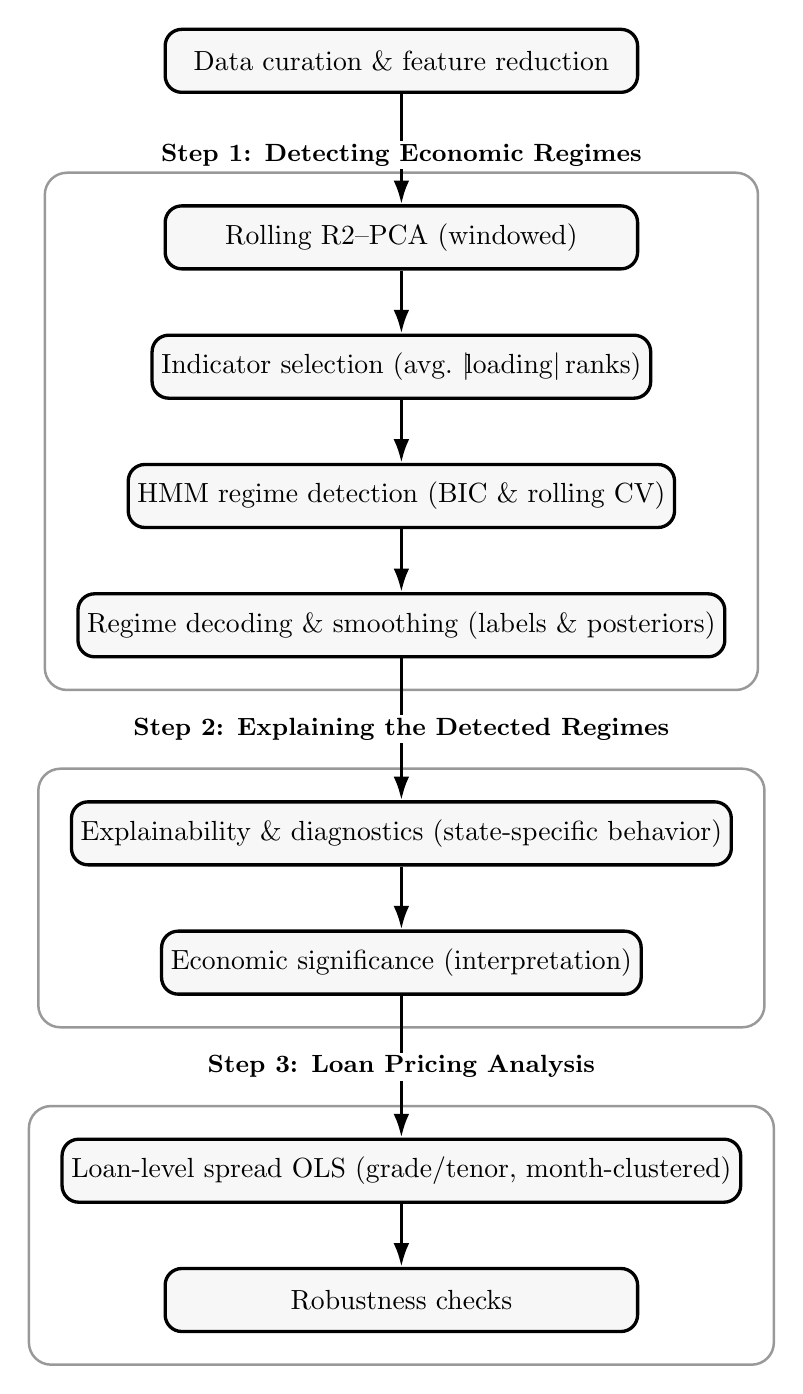
\begin{tikzpicture}[
  node distance = 8mm,
  box/.style      = {draw=black, rounded corners=6pt, very thick, fill=black!3,
                     align=center, minimum width=60mm, minimum height=8mm},
  arrow/.style    = {-{Latex[length=3mm,width=2mm]}, very thick},
  stepframe/.style= {draw=black!40, rounded corners=8pt, line width=0.9pt,
                     fill=none, inner sep=4mm}
]

% --- top box ---
\node[box] (data)   {Data curation \& feature reduction};

% make the first arrow longer and push Step 1 frame down a bit
\node[box, below=14mm of data]   (r2pca)  {Rolling R2--PCA (windowed)};
\node[box, below=of r2pca]       (select) {Indicator selection (avg.\ $|\!$loading$|\!$ ranks)};
\node[box, below=of select]      (hmm)    {HMM regime detection (BIC \& rolling CV)};
\node[box, below=of hmm]         (label)  {Regime decoding \& smoothing (labels \& posteriors)};

% increase space between Step 1 and Step 2 frames
\node[box, below=18mm of label]  (explain){Explainability \& diagnostics (state-specific behavior)};
\node[box, below=of explain]     (econ)    {Economic significance (interpretation)};

% increase space between Step 2 and Step 3 frames
\node[box, below=18mm of econ]   (ols)    {Loan-level spread OLS (grade/tenor, month-clustered)};
\node[box, below=of ols]         (rob)    {Robustness checks};

% arrows
\foreach \a/\b in {data/r2pca, r2pca/select, select/hmm, hmm/label,
                   label/explain, explain/econ, econ/ols, ols/rob}
  \draw[arrow] (\a) -- (\b);

% light step frames (behind)
\begin{scope}[on background layer]
  \node[stepframe, fit=(r2pca) (select) (hmm) (label)] (G1) {};
  \node[stepframe, fit=(explain) (econ)]               (G2) {};
  \node[stepframe, fit=(ols) (rob)]                    (G3) {};
\end{scope}

% step headers (keep same relative position; more room now due to larger gaps)
\node[fill=white, inner sep=1pt, font=\small\bfseries]
  at ([yshift=6pt] G1.north)
  {Step 1: Detecting Economic Regimes};

\node[fill=white, inner sep=1pt, font=\small\bfseries]
  at ($ (G1.south)!0.5!(G2.north) $)
  {Step 2: Explaining the Detected Regimes};

\node[fill=white, inner sep=1pt, font=\small\bfseries]
  at ($ (G2.south)!0.5!(G3.north) $)
  {Step 3: Loan Pricing Analysis};

\end{tikzpicture}%
}
\caption{Methodological framework and analysis flowchart. The analytical approach compresses the macro panel, selects indicators, and detects regimes in Step 1. It translates the detected regimes for interpretation in Step 2, and then conducts tests pricing effects using loan-level OLS, followed by robustness checks in Step 3.}
\label{fig:method_pipeline_linear_grouped}
\end{figure}

Ahead of the empirical analysis, we curate a broad set of monthly indicators and apply a transparent keyword filter (see table~\ref{tab:keyword_pipeline_dense}) to remove any irrelevant series. Subsequently we initiate the  regime detection process by running a rolling \(R^{2}\)-PCA that compresses the panel while preserving the evolving covariance structure. From these rolling decompositions we compute each indicator’s average \emph{absolute} loading and rank series by their scores accordingly. Secondly, we select the top eight observed indicators by this stability metric and feed them into a Gaussian HMM. The number of states is chosen by BIC with rolling cross-validation, and we decode monthly labels together with smoothed posterior probabilities to derive an empirically grounded regime signal that is statistically identifiable.
In a second step, we interpret the detected regimes. We fit a transparent surrogate decision tree to the HMM’s regime labels, which yields comprehensive split rules based on thresholds of the observed indicators and a ranking of variable importance. This clarifies which of the eight indicators move the economy into the contraction state and in what direction, providing an ordinal influence ordering. We then carry only the five most influential indicators that account for the majority of impurity reduction in the tree into the spread regressions as macro controls. Using exactly the variables that explain the regime mechanics keeps the pricing stage aligned with the identification stage, reduces macro indicator discretion, and improves parsimony. In this way we ensure a transparent, data-driven selection of macro controls that cleanly separates regime detection from pricing.


\subsection{Step 1: Detecting Economic Regimes}

%======================================================
\subsubsection{Rolling R2‑PCA}
\label{sec:R2PCA}
%======================================================

Principal‑component analysis (PCA) is commonly referred to as a standard device for compressing large macro‑financial information sets into a small number of common factors \citep{stock_macroeconomic_2002,bai_determining_2002,abdi_principal_2010}. Because naïve re‑estimation of PCA in rolling samples can produce erratic sign flips and rank re‑ordering of components, we implement the Robust Rolling PCA (R2‑PCA) procedure of \citet{hirsa_robust_2023}.\footnote{Details of the algorithmic implementation are outlined in \autoref{alg:r2pca}.} R2‑PCA performs an ordinary PCA in each window but then recursively aligns the resulting eigenvectors with those from the previous window via cosine‑similarity matching, correcting sign inversions and preserving the temporal identity of components even when local variance orderings change.\footnote{In the initial window the R2‑PCA eigenvectors coincide with the standard PCA solution. At each subsequent step, candidate eigenvectors from the new window are matched to those from the prior window by maximum absolute cosine similarity. Negatively aligned vectors are multiplied by $-1$ and the matched set is re‑ordered before projection. This stabilisation greatly improves interpretability when the panel spans multiple macro regimes.} We begin with a full‑sample PCA on the stationary $233\times 36$ panel described in Section~\ref{sec:data}. Let $\boldsymbol{\Sigma}$ denote the sample covariance matrix with ordered eigenvalues $\lambda_{1}\ge\cdots\ge\lambda_{d}$ and corresponding eigenvectors $\mathbf{p}_{1},\dots,\mathbf{p}_{d}$.  
The cumulative variance share after $k$ components is
\[
R^{2}(k)
= \frac{\sum_{i=1}^{k}\lambda_{i}}
       {\sum_{i=1}^{d}\lambda_{i}},
\qquad k=1,\dots,d.
\]
In our data the first seven components explain $R^{2}(7)=0.8286$ of total variance, which surpasses the 75\,\% heuristic of \citet{forni_generalized_2005} for meaningful economic inference and is visualized in Figure~\ref{fig:pc_cumvar}. Hence, we fix $K=7$ for the rolling analysis. Three considerations drive this choice. First, the incremental variance gain from adding an eighth component is small relative to the interpretability cost of tracking an additional factor across time. Second, when we feed $K=7$ into the R2‑PCA recursion, the window‑by‑window \emph{reconstruction} $R^{2}$ (Frobenius share of each 12‑month data block captured by the aligned seven‑dimensional subspace) remains high and never falls below $0.93$. Third, by using a common $K$ across windows we simplify the modelling of state‑spaces and real‑time updating through retaining a constant factor dimension to avoid spurious regime flags that could arise from changing the information set. To allow loadings to evolve with incoming data we re‑estimate PCA in a 12‑month trailing window that advances in step sizes of one month.  Denote by $\mathbf{X}_{t}\in\mathbb{R}^{12\times d}$ the standardized sample block whose final row corresponds to calendar month $t$ (with $d=36$ indicators). In each window we solve
\[
\min_{\mathbf F_{t},\,\mathbf P_{t}}
  \bigl\lVert \mathbf X_{t} - \mathbf F_{t}\mathbf P_{t}^{\top} \bigr\rVert_{F}^{2}
  \quad\text{s.t.}\quad
  \mathbf P_{t}^{\top}\mathbf P_{t} = \mathbf I_{K},
\]
with $K=7$. The resulting loading matrix $\mathbf P_{t}$ is \emph{R2‑aligned} with its predecessor from $t-1$ by maximum‑absolute cosine similarity. Any misaligned signs are flipped and the matched set is re‑ordered to preserve component identities through time \citep{hirsa_robust_2023}. Because consecutive windows overlap in eleven of twelve observations, we warm‑start the eigen-decomposition at $t$ with the aligned loadings from $t-1$, materially reducing computation time without affecting numerical convergence.\footnote{A similar computational benefit from warm starts in rolling matrix decompositions is documented by \citet{fan_projected_2016}.} From each window we retain the final‑month score vector, $\mathbf f_{t}=\mathbf F_{t}(12,:)$, thereby constructing a monthly factor panel $(\mathbf f_{t})_{t=1}^{T}$ that is synchronous with the raw indicators. For diagnostic purposes we compute a per‑window reconstruction statistic,
\[
R^{2}_{t}
= 1-\frac{\lVert \mathbf X_{t}-\hat{\mathbf X}_{t}\rVert_{F}^{2}}
           {\lVert \mathbf X_{t}\rVert_{F}^{2}},
\qquad
\hat{\mathbf X}_{t}=\mathbf F_{t}\mathbf P_{t}^{\top},
\]
whose empirical distribution (mean $0.97$, range $0.93$–$0.99$) confirms that seven components supply an adequate local approximation throughout the sample. Figure~\ref{fig:rolling_scores} plots the resulting R2‑aligned scores for $\text{PC}1$–$\text{PC}7$. Large, synchronized swings in the leading components coincide with well‑known macro stress episodes (global financial crisis, European sovereign debt crisis, COVID-19 pandemic), suggesting that a small number of dynamically aligned common factors can capture the majority of cyclical co‑movement in the underlying indicator set \citep{forni_generalized_2005, boivin_are_2006}. Subsequently, we translate these factors into a parsimonious set of macro drivers for the regime‑switching model.

\begin{figure}[H]
   \centering
   \includegraphics[width=.7\textwidth]{Graphics_P2P/fig_pc_cumvar.png} % cumulative‑variance plot
   \caption{Cumulative explained variance of principal components.  
   The dashed line marks the seven‑component cut‑off at which 82.86\,\% of total variance is reached. The horizontal red line depicts the 75\,\% target.}
   \label{fig:pc_cumvar}
\end{figure}

\begin{figure}[H]
   \centering
   \includegraphics[width=\textwidth]{Graphics_P2P/fig_rolling_scores.png} % rolling PC scores plot
   \caption{Seven rolling principal‑component scores.  
   Darker shades correspond to lower‑order components (PC1–PC3); lighter shades depict higher‑order components (PC4–PC7).}
   \label{fig:rolling_scores}
\end{figure}

Although the seven rolling PC scores summarize latent common factors, policy interpretation depends on identifying the observable indicators that contribute most. Thus, we use the seven PCs only to assess the rolling alignment and store for every window the absolute loading matrix \(\lvert\mathbf P_{t}\rvert\) of the macro indicators underlying the seven PCs. We average these macro indicators across windows and components,
\[
\bar{\ell}_{j}= \frac{1}{T}\sum_{t=1}^{T}\frac{1}{K}\sum_{k=1}^{K}\lvert P_{t,jk}\rvert,\qquad j=1,\dots,36,
\]
with \(T=222\) rolling windows.  
The eight macro indicators with the largest mean absolute loadings are reported in Table~\ref{tab:top8_loadings}. From the loading factor series we identify equity‑market volatility (\texttt{D084}, VIX) as the single strongest contributor. Labour‑market conditions follow subsequently with the four‑week moving average of initial unemployment claims (\texttt{D023}) and the unemployment rate for Hispanic workers (\texttt{D597}) load significantly, reflecting on evidence that P2P platforms attract borrowers from minority groups and workers with weaker attachment to traditional banking channels \citep{dolson_which_2021,jagtiani_fintech_2021,jagtiani_fintech_2018}. Two short‑term funding‑stress spreads, the 3‑month Treasury bill minus the effective fed‑funds rate (\texttt{D647}) and the 3‑month commercial‑paper minus fed‑funds spread (\texttt{D646}), are further identified as stress indicators in wholesale money markets and may represent the external cost of liquidity that alternative lenders face. Conversely, at a longer horizon, the Moody’s Aaa corporate–Treasury spread (\texttt{D365}) captures changes in fundamental credit risk premia. Real disposable personal income per capita (\texttt{D472}) and the apparel component of the CPI (\texttt{D110}) account as proxies for household purchasing power and cost‑of‑living pressures, which are two factors commonly found to shape both borrower demand and lenders’ required compensation in consumer lending markets \citep{agarwal_banks_2018,gross_liquidity_2002}.


\begin{table}[H]
\centering
\scriptsize
\caption{Top eight indicators by average absolute loading in rolling R2‑PCA}
\label{tab:top8_loadings}
\begin{threeparttable}
\begin{tabular}{llr}
\toprule
\textbf{Code} & \textbf{Indicator} & \textbf{Avg.\,$|$loading$|$} \\
\midrule
D084 & VIX (equity‐market volatility)                      & 0.1731 \\
D023 & Initial Claims, 4‑week Moving Avg.                  & 0.1638 \\
D597 & Unemployment Rate – Hispanic                        & 0.1579 \\
D647 & 3‑M T‑Bill minus Fed‑Funds Spread                   & 0.1577 \\
D646 & 3‑M Commercial Paper minus Fed‑Funds Spread         & 0.1512 \\
D472 & Real Disposable Income per Capita                   & 0.1504 \\
D110 & CPI Apparel                                         & 0.1503 \\
D365 & Moody’s Aaa Corp. Yield minus 10‑Y Treasury         & 0.1474 \\
\bottomrule
\end{tabular}
\begin{tablenotes}[flushleft]\footnotesize
\item \emph{Notes}: In each 12‑month rolling window the absolute loadings of the seven retained principal components are averaged across components. The resulting \(36\times 222\) matrix (36 indicators, 222 windows) is then averaged over all windows to obtain \(\bar{\ell}_{j}\) for each indicator \(j\). The eight series with the largest \(\bar{\ell}_{j}\) values are listed above and fed into the Hidden‑Markov regime detector. All loadings are computed on standardised input series, so magnitudes are directly comparable across indicators.
\end{tablenotes}
\end{threeparttable}
\end{table}


%======================================================
\subsubsection{Regime Detection via Hidden Markov Models}
\label{sec:hmm}
%======================================================

To capture switches between distinct macro-credit states we model the eight selected macro indicators as emissions from a finite Hidden Markov Model (HMM) with multivariate Gaussian output densities. Let \(S_{t}\in\{1,\ldots,K\}\) denote the unobserved regime at month \(t\) and \(\mathbf{x}_{t}\in\mathbb{R}^{d}\) the corresponding observation vector, where \(d=8\).  
Conditional on \(S_{t}=k\), we assume  
\[
\mathbf{x}_{t}\;\vert\;S_{t}=k \;\sim\;
\mathcal{N}\!\bigl(\boldsymbol{\mu}_{k},\,
\mathrm{diag}(\boldsymbol{\sigma}^{2}_{k})\bigr),
\qquad k=1,\ldots,K,
\]
where diagonal covariance matrices mitigate the curse of dimensionality in short rolling windows \citep{tomarchio_parsimonious_2022}. While this assumption constrains within-regime indicator correlations, it provides computational stability and interpretability. Regime dynamics obey a first-order Markov chain with transition matrix \(\mathbf{P}=(P_{ij})_{i,j=1}^{K}\). The estimation is proceeded each month on an expanding window via the expectation–maximisation (EM) algorithm after \(z\)-scoring the indicators. State means are initialized by R2-KMeans \citep{holmes_robust_2024} and form the basis for the uniform transition matrix, which is subsequently re-estimated in iterations until the increase in the observed-data log-likelihood falls below \(10^{-6}\). To maintain time-consistent labels in the rolling estimation, the current month’s Gaussian components are matched to those of the previous month by solving a linear assignment on a cost that combines differences in component means and (diagonal) covariances. The resulting mapping fixes regime indices across months \citep{hirsa_robust_2024}. For monitoring, we archive one-step negative log-likelihoods in a 12-month sliding buffer and flag observations in the upper $5\%$. Because the likelihood of a Hidden Markov Model increases mechanically with the number of latent states, we combine a penalized in-sample criterion with an explicit out-of-sample test. For the in-sample leg we evaluate candidate models with \(K=2,\ldots,4\) on a fixed training window, spanning June 2007 to May 2010, and compute the Bayesian Information Criterion,
\[
\mathrm{BIC}(K)= -2\,\ell\!\bigl(\widehat{\boldsymbol{\theta}}_{K}\bigr)
                 + p_{K}\,\ln N,
\]
where \(\ell(\cdot)\) is the maximised log-likelihood, \(N\) is the number of training observations, and \(p_{K}=(K-1)+K(K-1)+2Kd\) is the parameter count comprising initial probabilities, transition intensities, and regime-specific means and variances.\footnote{The possible state space in the training window is based on Merrill Lynch's Investment Clock \citep{greetham_special_2004}, defining $\mathcal{Z} = \{ Reflation, Recovery, Overheat, Stagflation\}$.} Table~\ref{tab:ic_cv} reports the information criteria alongside the rolling out-of-sample scores, and Figure~\ref{fig:hmm_threepanel}\, visualizes the same diagnostics across $K\in\{2,3,4\}$.
Within this window the BIC attains its minimum at two states, with higher-order specifications penalized for over-parameterization. To guard against the possibility that a higher-order model may generalize better even if it is favored in-sample, we implement a rolling out-of-sample cross-validation scheme. Starting from the same cut-off (May 2010), we roll the estimation boundary forward in quarterly steps.  In each fold the model is re-estimated on the expanding history up to the fold-start and evaluated on the next twelve months of data. The resulting one-year cumulative log-likelihoods are averaged across folds. The mean out-of-sample score is denoted by \(\mathrm{CV}(K)\). In the observation sample \(\mathrm{CV}(K)\) peaks at two states, thereby supporting the model parsimony suggested by the BIC, which is congruent with findings by \cite{maalaoui_chun_credit_2014} for economic episodes of high or low credit spreads. Accordingly, we set $K^{\star}=2.$

\begin{table}[H]
\centering
\caption{Information criteria and out‑of‑sample CV log‑likelihood for $K=2$–$4$}
\label{tab:ic_cv}
\begin{tabular}{rrrr}
\toprule
\textbf{$K$} & \textbf{BIC} & \textbf{AIC} & \textbf{Mean CV log‑likelihood} \\
\midrule
2 & 1\,168.93 & 1\,113.50 & $-485.53$ \\
3 & 1\,767.88 & 1\,679.21 & $-645.38$ \\
4 & 1\,592.17 & 1\,467.07 & $-967.57$ \\
\bottomrule
\end{tabular}
\begin{minipage}{.78\linewidth}
\vspace{2pt}\footnotesize\emph{Notes}:  
BIC and AIC are calculated on the fixed training window (Jun 2007–May 2010).  
The CV column reports the mean one‑year‑ahead cumulative log‑likelihood from a quarterly rolling cross‑validation.  
Lower (higher) values indicate a better fit for the information criteria (CV log‑likelihood).
\end{minipage}
\end{table}

After fixing the number of states, the model is re‑estimated each month via an expanding‑window approach. The estimation begins with a $24$‑month warm‑up segment and proceeds by warm‑starting the EM routine at the parameter values of the preceding month. This strategy reduces computation time by roughly an order of magnitude relative to cold starts and produces smoother parameter estimates. For every update we obtain filtered regime probabilities via the forward algorithm and assign point labels by maximum a‑posteriori choice \citep{hamilton_new_1989}. Negative log‑likelihoods are archived in a twelve‑month sliding buffer with an observation being flagged whenever its likelihood falls into the upper $5\%$ tail of that buffer.

%------------------------------------------------
% HMM diagnostics and monitoring (3 panels)
%------------------------------------------------
\begin{figure}[H]
\centering

% --- Top: full-width decoded labels ---
\begin{subfigure}[t]{0.85\linewidth}
  \centering
  \includegraphics[width=\linewidth]{Graphics_P2P/regime_labels.png}
  \caption{Decoded hard regime sequence}\label{fig:path_sub}
\end{subfigure}

\vspace{6pt} % small vertical gap

% --- Bottom row: two half-width panels ---
\begin{subfigure}[t]{0.54\linewidth}
  \centering
  \includegraphics[width=\linewidth]{Graphics_P2P/cv_selection.png}
  \caption{Rolling-window CV log-likelihood}\label{fig:cv_sub}
\end{subfigure}\hfill
\begin{subfigure}[t]{0.44\linewidth}
  \centering
  \includegraphics[width=\linewidth]{Graphics_P2P/smoothed_state_probs.png}
  \caption{Smoothed posterior regime probabilities}\label{fig:prob_sub}
\end{subfigure}

\caption{Model-selection diagnostics and real-time monitoring for the preferred two-state HMM.}
\begin{minipage}{0.94\linewidth}
\footnotesize
Panel (a) shows the decoded hard regime sequence (June 2007–March 2025).  
Panel (b) reports the mean one-year-ahead cumulative log-likelihood from a quarterly rolling cross-validation across $K\in\{2,3,4\}$, which favours $K=2$.  
Panel (c) plots the smoothed posterior probabilities $\Pr(S_t=k\,|\,\mathcal{F}_T)$. Values near one (zero) indicate months assigned almost exclusively to Regime 1 (Regime 2).  
The dashed vertical lines mark contraction phases identified between June 2007 and March 2025.
\end{minipage}
\label{fig:hmm_threepanel}
\end{figure}



%======================================================
\subsection{Step 2: Explaining the Detected Regimes}
\label{sec:explain}
%======================================================

\subsubsection{State‑Specific Interpretation}

Because each hidden state is parameterized by a multivariate normal density, the estimated regime‑specific means and diagonal variances offer an immediate view of conditional levels and dispersion. For regime \(k\), the vector of conditional expectations \(\boldsymbol{\mu}_{k}\) shows, for instance, whether labour‑market- or funding‑stress spreads tend to be elevated. Contrarily, the diagonal of \(\boldsymbol{\Sigma}_{k}\) quantifies the within‑regime volatility of every indicator.

\begin{table}[H]
\centering
\scriptsize
\caption{Regime‑conditional means and variances of the macro drivers}
\label{tab:state_mu_sigma}
\begin{threeparttable}
\begin{tabular}{lrrrrrrrr}
\toprule
 & \textbf{D084} & \textbf{D023} & \textbf{D597} & \textbf{D647} & \textbf{D646} & \textbf{D472} & \textbf{D110} & \textbf{D365} \\ \midrule
\multicolumn{9}{l}{\textbf{Panel A: Means $\boldsymbol{\mu}_{k}$}}\\
Regime 1 (accomm.) & $-0.265$ & $-0.185$ & $-0.212$ & $-0.029$ & $-0.269$ & $0.099$ & $-0.010$ & $-0.019$\\
Regime 2 (restrict.) & $0.578$ & $0.404$ & $0.464$ & $0.064$ & $0.587$ & $-0.216$ & $0.023$ & $0.041$\\[4pt]
\multicolumn{9}{l}{\textbf{Panel B: Variances $\boldsymbol{\sigma}_{k}^{2}$}}\\
Regime 1 (accomm.) & $0.485$ & $0.002$ & $0.063$ & $0.208$ & $0.206$ & $0.191$ & $0.496$ & $0.514$\\
Regime 2 (restrict.) & $1.638$ & $2.943$ & $2.733$ & $2.725$ & $2.232$ & $2.700$ & $2.100$ & $2.059$\\
\bottomrule
\end{tabular}
\begin{tablenotes}[flushleft]\footnotesize
\item \emph{Notes}: Means and variances are computed on $z$‑scored observations assigned to each decoded regime (Jun 2007–Mar 2025).  
Regime 1 corresponds to the accommodative phase (share 74.6 \%), Regime 2 to the restrictive phase (share 25.4 \%).
\end{tablenotes}
\end{threeparttable}
\end{table}

\begin{figure}[H]
\centering
\begin{subfigure}{.48\linewidth}
  \includegraphics[width=\linewidth]{Graphics_P2P/corr_regime1.png}
  \caption{Accommodative Regime 1}
\end{subfigure}\hfill
\begin{subfigure}{.48\linewidth}
  \includegraphics[width=\linewidth]{Graphics_P2P/corr_regime2.png}
  \caption{Restrictive Regime 2}
\end{subfigure}
\caption{Pairwise correlation matrices of the eight macro drivers by regime.  
In the restrictive phase stronger co‑movement emerges between unemployment claims (D023), Hispanic unemployment (D597) and equity‑market volatility (D084), alongside tight linkages among funding‑stress spreads (D646, D647) and the Aaa–Treasury spread (D365).}
\label{fig:corr_regime}
\end{figure}

As shown in Table~\ref{tab:state_mu_sigma}, the regime-conditional moments indicate the alignment of the second state with a restrictive configuration. The positive means of the macros factor inputs in Regime~2 imply that labour-market stress, funding pressure, and credit-risk premia are simultaneously above their accommodative levels. By contrast, Regime~1 exhibits muted or slightly negative means on these indicators and a positive mean for \texttt{D472}, consistent with eased economic conditions. The variance profiles confirm this distinction as the within-regime dispersion is uniformly higher in Regime~2 (often by an order of magnitude), signalling inherently more volatile macro-financial dynamics in restrictive periods. The correlation heat maps in Figure~\ref{fig:corr_regime} further clarify the structure of each state. In the accommodative regime, cross-indicator co-movements are weak to moderate. However, in the restrictive regime, two clusters emerge: (i) a labour-and-volatility block, with tight positive correlations among \texttt{D023}, \texttt{D597}, and \texttt{D084}, and (ii) a funding-stress block linking \texttt{D646}, \texttt{D647}, and \texttt{D365}. These stress factors co-move negatively with household-demand proxies (\texttt{D472}, \texttt{D110}), consistent with deficits in income and consumption during economic downturns. The joint rise in labour distress, market volatility, and funding premia in combination with depressed real income therefore provides an economic interpretation of the restrictive state as a generalized episode of financial distress.

Beyond first‑ and second‑order moments, in the restrictive regime both labour‑market stress measures (\texttt{D023}, \texttt{D597}) exhibit pronounced right‑skew, reflecting surges during downturns. Short‑term funding‑stress spreads (\texttt{D647}, \texttt{D646}, \texttt{D365}) shift upward and widen, while risk sentiment deteriorates as the VIX (\texttt{D084}) moves to a markedly higher level, thereby displaying thicker right tail skewness. In contrast, real disposable income per capita (\texttt{D472}) shows a left‑shift with a fat lower tail, while the CPI apparel series (\texttt{D110}) moderates, pointing to reduced discretionary spending. Hence, the distributional evidence corroborates the insight of heightened risk, tighter funding, and strained household cash flows during restrictive macro‑credit phases \citep{gambacorta_impact_2020}.

\begin{figure}[H]
\centering
\includegraphics[width=\linewidth]{Graphics_P2P/indicator_boxplots.png}
\caption{Conditional distributions of the eight macro drivers by decoded regime (Tukey box‑plots with outliers).  
The restrictive phase (Regime 2) features higher volatility (D084), elevated unemployment claims and Hispanic unemployment (D023, D597), wider funding‑stress spreads (D646, D647) and credit‑risk premia (D365), alongside lower real disposable income (D472).}
\label{fig:box_regime}
\end{figure}

While the HMM’s posterior probabilities are informative, their latent structure must be translated into operational rules to become further interpretable. To obtain a representation of the regime switches and the macro factors that contribute most, we fit a family of shallow classification trees to the regime labels, using exactly the eight macro‑financial predictors that feed the HMM. The hyper‑parameter grid spans depths 2–4 with minimum leaf sizes 5, 10, 20. For every combination we record five‑fold stratified cross‑validated (CV) accuracy and retain all models whose mean CV accuracy lies within $2\%$ of the global best. The resulting Pareto frontier contains two candidates of particular interest. A \textit{depth‑2, three‑leaf tree} with a mean CV accuracy of 93.9 \%, offering the most concise set of rules possible. By allowing one additional level, we yield a \textit{depth‑3 tree with five terminal nodes} whose accuracy improves to 94.0\%. Although the numerical gain is modest, the extra branch supports in keeping the rule set easily interpretable. Figure~\ref{fig:manual_tree} depicts the preferred depth‑3 tree.

%------------------------------------------------
%  Manually fine‑tuned decision tree (depth 3)
%------------------------------------------------
\begin{figure}[H]
  \centering
  \includegraphics[width=.95\linewidth]{Graphics_P2P/manual_tree_depth3.png}
  \caption{Fine‑tuned decision tree (depth 3, five leaves).  
  The root split is the standardized Hispanic unemployment rate (\texttt{D597}). Months with \(\texttt{D597}>1.15\sigma\) are labeled restrictive (Regime 2). If \(\texttt{D597}\le 1.15\sigma\), the tree evaluates the standardized four-week moving average of initial claims (\texttt{D023}). Months with \(\texttt{D023}\le -0.26\sigma\) are also classified as restrictive. When labour-market stress is only moderate on both indicators, the commercial-paper–fed-funds spread (\texttt{D646}) provides the deciding split.  
  The tree attains an average five‑fold CV accuracy of 94.0 \%.}
  \label{fig:manual_tree}
\end{figure}

The depth‑3 topology translates the latent‑state logic into the four mutually exclusive threshold rules listed in Table~\ref{tab:robust_rules}. Relative to its depth‑2 counterpart, the additional split on the commercial‑paper–fed‑funds spread (\texttt{D646}) reduces false accommodative signals by roughly $4\%$ of the sample, underscoring the informational content of short‑term funding conditions during regime transitions.\footnote{Importantly, all thresholds are expressed in regime‑standardised \(\sigma\)‑units, rendering the rules invariant to future sample extensions and therefore suitable for out‑of‑sample monitoring.}

%------------------------------------------------
%  Core decision rules that survive the grid search
%------------------------------------------------
\begin{table}[H]
\centering
\caption{Decision rules from the fine‑tuned depth‑3 tree}
\label{tab:robust_rules}
\begin{threeparttable}
\begin{tabular}{p{0.70\linewidth}c}
\toprule
\textbf{Decision rule (standardised units)} & \textbf{Predicted regime}\\
\midrule
$\texttt{D597} > 1.15$                                                                                    & Restrictive (2)\\[2pt]

$\texttt{D597} \le 1.15\;\wedge\;\texttt{D023} \le -0.26$                                                 & Restrictive (2)\\[2pt]

$\texttt{D597} \le 1.15\;\wedge\;\texttt{D023} > -0.26\;\wedge\;\texttt{D646} \le 0.39$                   & Accommodative (1)\\[2pt]

$\texttt{D597} \le 1.15\;\wedge\;\texttt{D023} > -0.26\;\wedge\;\texttt{D646} > 0.39$                     & Restrictive (2)\\
\bottomrule
\end{tabular}
\begin{tablenotes}[flushleft]\footnotesize
\item \emph{Notes}: Rules correspond to the depth‑3 tree plotted in Figure \ref{fig:manual_tree}.  
Variables are expressed in regime‑standardised units; thresholds therefore remain invariant under sample extensions.  
The rule set attains a mean five‑fold CV accuracy of 94.0\%.
\end{tablenotes}
\end{threeparttable}
\end{table}


%======================================================
\subsubsection{Economic significance}
%======================================================

From the regime partitions over the period June 2007–March 2025 we observe posterior state probabilities that assign 74.6\% of months to regime 1 and the remaining 25.4\% form several short‑lived but distinct restrictive episodes. In the restrictive regime 2 relative to its historical mean, the labour‑market stress measures (\texttt{D023}, \texttt{D597}) rise by more than one standard deviation, consistent with the inception of distressed labour markets during heightened economic turmoil. Similarly, the short‑term funding spreads (\texttt{D646}, \texttt{D647}) both shift upward, while market‑based risk sentiment increases as the VIX (\texttt{D084}) remains in the top quartile of its empirical distribution consistent with a flight‑to‑quality behavior \citep{caballero_collective_2008, baele_flights_2020}. In contrast, in the accommodative regime 1 we observe normalization in each macro time series with indicators returning to or below their average trend. This regime recurs in three extended clusters (2010–2012, 2013–2018, 2023–2025) consistent with patterns for surges in household debt, characterized by 3–4-year run-ups followed by reversal and weaker economic growth \citep{mian_household_2017}. Based on the feature importance ranking of the surrogate tree in figure~\ref{fig:manual_tree}, we can observe that regime shifts are led by labour‑market stress (\texttt{D597}, \texttt{D023}), short‑term liquidity (\texttt{D646}, \texttt{D647}), and equity‑market volatility \texttt{D084}. At the root node split, the Hispanic unemployment rate is determined as the essential economic contraction indicator with values above \(1.15\sigma\) signaling a restrictive month irrespective of other conditions. If \texttt{D597} is below this threshold, pronounced dislocations in \texttt{D023} ($\le -0.26\sigma$) are sufficient to classify the month as restrictive. If both labour-market signals remain within their thresholds, classification rests on money-market conditions. The CP–fed-funds differential is then found to provide the marginal separator, with $\texttt{D646}>0.39\sigma$ indicating residual stress consistent with the restrictive state and $\texttt{D646}\le 0.39\sigma$ mapping to the accommodative state.

\subsection{Step 3: Loan Pricing Analysis}
\subsubsection{Loan‑Level Credit‑Spread Regressions}
\label{subsec:reg_setup}

To investigate, whether the decoded macro‑regime signal and the selected macro drivers have any impact on primary‑market pricing in P2P lending, we estimate cross‑sectional regressions of loan‑level credit spreads on a monthly basis over the time span from 2007 to 2012. For loan \(i\) issued in month \(t\),
\[
\textit{credit\_spread}_{i,t}
   = \alpha 
   + \beta_{1}\,\textit{Contraction}_{t}
   + \beta_{2}^{\top}{m}_{t}
   + \gamma^{\top}{x}_{i,t}
   + \varepsilon_{i,t},
\]
where \(\textit{Contraction}_{t}\) equals 1 if the Hidden Markov Model classifies month \(t\) as \emph{restrictive} (Regime~2) and 0 otherwise, \(m_{t}\) is the vector of five macro drivers identified in Section~\ref{sec:explain} (initial unemployment claims \(D023\), Hispanic unemployment rate \(D597\), equity‑market volatility \(D084\), the 3‑month T‑bill less fed‑funds spread \(D647\), and the commercial‑paper less fed‑funds spread \(D646\)), and \(x_{i,t}\) contains borrower‑level controls.\footnote{These variables include the contractual maturity in months (\(\textit{term\_num}\)), debt‑to‑income ratio (\(\textit{dti}\)), and \(\log(\textit{annual\_inc})\)).} As in \cite{foo_discovering_2023} we report two complementary designs. (\emph{i}) Initially we estimate grade‑specific regressions within each letter grade \(g\in\{\text{A},\ldots,\text{G}\}\) using the full set of eligible loans in that grade, with \(x_{i,t}\) as above. (\emph{ii}) Subsequently, we test term‑specific regressions by pooled fits within each tenor \(h\in\{36,60\}\) months that include the full set of grade fixed effects in \(x_{i,t}\). Estimation proceeds by ordinary least squares (OLS) with Huber–White standard errors clustered at the calendar‑month level, which accommodates heteroskedasticity across loans and serial correlation induced by month‑level regressors shared within a cross‑section \citep{moulton_illustration_1990,petersen_estimating_2009}. The dependent variable \(\textit{credit\_spread}_{i,t}\) is defined as the contractual coupon minus a risk‑free benchmark that matches the existing loan maturities.\footnote{We use the three‑year constant‑maturity Treasury yield for 36‑month loans and the five‑year yield for 60‑month loans (FRED series \texttt{DGS3} and \texttt{DGS5}). All monthly quotes are converted to decimals and sampled at month‑end.}

%======================================================
\section{Empirical Results and Discussion}
\label{sec:results}

%------------------------------------------------
\subsection{Grade-specific regressions}
\label{subsec:grade_regs}
%------------------------------------------------

The decoded regimes in the observation period (June~2007–December~2012) appear to move systematically with the average primary‑market spreads as indicated by Figure~\ref{fig:avg_spread_regime}. Restrictive episodes are associated with discrete upward shifts in spreads across all grades, with larger level increases for lower‑rated buckets. Table~\ref{tab:grade_regress} reports separate cross-sectional regressions of loan credit spreads on the restrictive-regime indicator and macro drivers for Grades~A–G.

\begin{figure}[H]
  \centering
  \includegraphics[width=\linewidth]{Graphics_P2P/avg_spread_by_grade_term.png}
  \caption{Monthly average credit spreads by grade and term (Jun~2007–Dec~2012).}
  \label{fig:avg_spread_regime}
\end{figure}

\begin{table}[H]
\centering
\scriptsize
\caption{Credit-spread regressions by credit grade (Jun~2007–Dec~2012)}
\label{tab:grade_regress}
\begin{threeparttable}
\begin{tabular}{lrrrrrrr}
\toprule
 & \multicolumn{1}{c}{\textbf{A}} & \multicolumn{1}{c}{\textbf{B}} & \multicolumn{1}{c}{\textbf{C}} &
   \multicolumn{1}{c}{\textbf{D}} & \multicolumn{1}{c}{\textbf{E}} & \multicolumn{1}{c}{\textbf{F}} &
   \multicolumn{1}{c}{\textbf{G}} \\
\midrule
\multicolumn{8}{l}{\textit{Macro variables}} \\[2pt]
Contraction
  & \,0.006$^{*}$  & \,0.008$^{***}$ & \,0.005$^{**}$ & \,0.011$^{***}$ &
    \,0.017$^{***}$ & \,0.018$^{***}$ & \,0.021$^{***}$ \\
  & (0.003) & (0.003) & (0.002) & (0.004) & (0.006) & (0.006) & (0.005) \\[4pt]
Init.\ claims 4-wk MA ($D023$)
  & \,0.035$^{***}$ & \,0.051$^{***}$ & \,0.048$^{***}$ & \,0.073$^{***}$ &
    \,0.102$^{***}$ & \,0.113$^{***}$ & \,0.115$^{***}$ \\
  & (0.007) & (0.008) & (0.007) & (0.011) & (0.018) & (0.023) & (0.021) \\[4pt]
Unemp.\ rate Hisp.\ ($D597$)
  & $-0.003^{***}$ & $-0.006^{***}$ & $-0.007^{***}$ & $-0.011^{***}$ &
    $-0.014^{***}$ & $-0.015^{***}$ & $-0.016^{***}$ \\
  & (0.001) & (0.001) & (0.001) & (0.001) & (0.002) & (0.002) & (0.002) \\[4pt]
VIX ($D084$)
  & $-0.000$ & $-0.002$ & $-0.003$ & $-0.003$ &
    $-0.003$ & $-0.002$ & $-0.005$ \\
  & (0.002) & (0.004) & (0.003) & (0.006) & (0.008) & (0.009) & (0.009) \\[4pt]
3-m T-bill–FF ($D647$)
  & $-0.045$ & $-0.042$ & $-0.075$ & $-0.084$ & $-0.154$ & $-0.154$ & $-0.210$ \\
  & (0.040) & (0.055) & (0.055) & (0.085) & (0.127) & (0.135) & (0.141) \\[4pt]
CP–FF ($D646$)
  & $-0.004$ & $-0.032$ & $-0.050^{**}$ & $-0.079^{*}$ &
    $-0.094^{*}$ & $-0.109^{*}$ & $-0.044$ \\
  & (0.016) & (0.026) & (0.024) & (0.040) & (0.056) & (0.060) & (0.056) \\[6pt]
Observations & 20\,186 & 29\,570 & 18\,987 & 12\,115 & 5\,849 & 2\,322 & 571 \\
Adj.\ $R^{2}$ & 0.136 & 0.275 & 0.498 & 0.618 & 0.588 & 0.612 & 0.610 \\
\bottomrule
\end{tabular}
\begin{tablenotes}[flushleft]\footnotesize
\item \emph{Notes}: The dependent variable is the quoted credit spread in percentage points (pp); e.g., 0.010 = 100\,bp. All regressions include maturity in months (\textit{term\_num}), borrower debt-to-income (\textit{dti}), and $\log(\textit{annual\_inc})$ (coefficients omitted). Standard errors clustered by issuance month are shown in parentheses. $^{***}$, $^{**}$, and $^{*}$ denote significance at the 1\%, 5\%, and 10\% levels, respectively. Series enter in non-standardized units. The regime indicator is a 0–1 dummy, hence $\hat\beta(\text{Contraction})$ gives the level shift when the month is classified as restrictive. $D023$ (initial claims) and $D084$ (VIX) are percentage changes (\textit{pct}) in decimal units; a $+1\%$ monthly change corresponds to $\Delta X=0.01$. $D597$ (Hispanic unemployment) is the \textit{first difference} of a percentage rate (\textit{diff}); $\Delta X=0.1$ equals a $+0.1$\,pp monthly change. $D646$ (CP–FF) and $D647$ (T-bill–FF) are \textit{level differentials} in percent; $\Delta X=0.10$ corresponds to a $+10$\,bp move. Coefficients map to spread changes via $\Delta\text{spread}=\hat\beta\,\Delta X$ (in pp). For \textit{pct} variables, multiply $\hat\beta$ by $0.01$ to obtain the pp change for a $+1\%$ move. For \textit{diff} variables, multiply by $0.1$ for a $+0.1$\,pp change; for \textit{Percent} differentials, multiply by $0.10$ for a $+10$\,bp move. Exemplarily, for Grade D, $\hat\beta(D023)=0.073$ implies $\approx 0.073\times 0.05=0.0037$ (37\,bp) for a $+5\%$ rise in claims.
\end{tablenotes}
\end{threeparttable}
\end{table}

Overall, the observed effect is positive for all grades and generally rising across the rating band. From this observation we infer a uniform pass‑through of macro stress that is steeper for riskier borrowers.\footnote{To test whether regime months coincide with different loan mixes, we have further tested the composition of the loan panel. Results in appendix Table~\ref{tab:mix_by_regime} show grade shares to be similar across regimes, while the 36m/60m mix shifts. A Pearson $\chi^2$ test rejects independence for both grade- and term–regime. Hence, we have conditioned the pricing models on grade/term and included borrower controls to identify outcomes comes from within-grade/within-term variation. Through this specification we can ensure that the reported regime and macro coefficients are not mechanically driven by composition shifts.} This finding coincides with \cite{nigmonov_macroeconomic_2022} who find P2P credit spreads to react with stronger magnitudinal effects in lower grade loans during changes in macro-economic conditions. In relative terms, the point estimates rise from roughly $+0.6\%$ to $+2.1\%$ (about $+60$ to $+210$ basis points), with statistical significance for Grades~A–G. From the initial results we can corroborate two dynamics of credit spread changes observed by \cite{foo_discovering_2023} in P2P lending markets. First, we find the labor-stress related macro determinants in form of initial jobless claims (\texttt{D023}) to carry positive and significant coefficients in every grade, with semi‑elasticities that generally increase with borrower risk. Second, the unemployment proxy (\texttt{D597}) is negatively associated with spreads across grades in this sample window. By contrast, equity‑market volatility (\texttt{D084}) is small and statistically indistinct from zero, while the money‑market stress measures (\texttt{D646}, \texttt{D647}) are generally negative and weakly estimated, with no systematic sign reversal for lower grades. 

%------------------------------------------------
\subsection{Maturity‑specific regressions}
\label{subsec:term_regs}
%------------------------------------------------
To assess horizon dependence in regime pass‑through, we pool loans by tenor and include the full set of grade fixed effects alongside borrower controls.  
Table~\ref{tab:term_regress} summarizes the estimates for 36‑ and 60‑month contracts.

\begin{table}[H]
\centering
\scriptsize
\caption{Credit-spread regressions by loan maturity (Jun~2007–Dec~2012)}
\label{tab:term_regress}
\begin{threeparttable}
\begin{tabular}{lrr}
\toprule
 & \multicolumn{1}{c}{\textbf{36-month}} & \multicolumn{1}{c}{\textbf{60-month}} \\
\midrule
\multicolumn{3}{l}{\textit{Macro variables}} \\[2pt]
Contraction 
  & \,0.0059$^{**}$ & \,0.0133$^{***}$ \\
  & (0.002) & (0.003) \\[4pt]
Init.\ claims 4-wk MA ($D023$) 
  & \,0.0471$^{***}$ & \,0.0903$^{**}$ \\
  & (0.007) & (0.043) \\[4pt]
Unemp.\ rate Hisp.\ ($D597$) 
  & $-0.0057^{***}$ & $-0.0131^{***}$ \\
  & (0.001) & (0.004) \\[4pt]
VIX ($D084$) 
  & $-0.0019$ & $-0.0019$ \\
  & (0.003) & (0.007) \\[4pt]
3-m T-bill–FF ($D647$) 
  & $-0.0487$ & $-0.1338$ \\
  & (0.047) & (0.120) \\[4pt]
CP–FF ($D646$) 
  & $-0.0371^{*}$ & $-0.0500$ \\
  & (0.022) & (0.049) \\[6pt]
Grade fixed effects & Yes & Yes \\[2pt]
Borrower controls ($\textit{dti}$, $\log \textit{inc}$) & Yes & Yes \\[2pt]
Observations & 69\,013 & 20\,587 \\
Adj.\ $R^{2}$ & 0.904 & 0.896 \\
\bottomrule
\end{tabular}
\begin{tablenotes}[flushleft]\footnotesize
\item \emph{Notes}: The dependent variable is the contractual coupon minus the matched Treasury yield, measured in \emph{percentage points} (pp); e.g., 0.010 = 1.0\,pp = 100\,bp. Both regressions include seven grade dummies, borrower debt-to-income (\textit{dti}), and $\log(\textit{annual\_inc})$ (coefficients omitted). Monthly cluster-robust standard errors are in parentheses. $^{***}$, $^{**}$, and $^{*}$ indicate significance at the 1\%, 5\%, and 10\% levels, respectively. Series enter in non-standardized units. The regime indicator is a 0–1 dummy, hence $\hat\beta(\text{Contraction})$ gives the level shift when the month is classified as restrictive. $D023$ (initial claims) and $D084$ (VIX) are \textit{percentage changes} (\textit{pct}) in decimal units; a $+1\%$ monthly change corresponds to $\Delta X=0.01$. $D597$ (Hispanic unemployment) is the \textit{first difference} of a percentage rate (\textit{diff}); $\Delta X=0.1$ equals a $+0.1$\,pp monthly change. $D646$ (CP–FF) and $D647$ (T-bill–FF) are \textit{level differentials} in percent; $\Delta X=0.10$ corresponds to a $+10$\,bp move. Coefficients map to spread changes via $\Delta\text{spread}=\hat\beta\,\Delta X$ (in pp). For \textit{pct} variables, multiply $\hat\beta$ by $0.01$ to obtain the pp change for a $+1\%$ move. For \textit{diff} variables, multiply by $0.1$ for a $+0.1$\,pp change; for \textit{Percent} differentials, multiply by $0.10$ for a $+10$\,bp move. For illustration, the 60-month estimate $0.0133$ implies an average spread increase of $0.0133$\,pp ($=133$\,bp) in restrictive months, versus $0.0059$\,pp ($=59$\,bp) for 36-month loans.
\end{tablenotes}
\end{threeparttable}
\end{table}

After absorbing grade heterogeneity, restrictive months are associated with higher spreads at both horizons, with a larger effect for five‑year loans (approximately $+133$~bp) than for three‑year loans (approximately $+59$~bp). The detected macro fundamentals remain priced with initial jobless claims (\texttt{D023}) widen coupons, and the Hispanic unemployment rate (\texttt{D597}) is negatively associated with spreads in both tenors. Money-market stress proxies are generally negative and weakly estimated. The commercial-paper–fed-funds spread ($D646$) is marginally negative for 36-month loans (10\% level) and insignificant for 60-month loans. The 3-month T-bill–fed-funds spread ($D647$) is not significant at either horizon. Equity-market volatility ($D084$) is small and statistically indistinguishable from zero.


%------------------------------------------------
\subsection{Economic interpretation and implications for platform pricing}
\label{subsec:econ_interp}
%------------------------------------------------
The cross‑sectional results indicate a broad expansion of risk premia in restrictive months across credit grades and terms consistent with regular findings in traditional bond markets \citep{gilchrist_credit_2012, collin-dufresn_determinants_2001}. The regime dummy is uniformly positive across grades and generally increases with borrower risk by approximately $+60$~bp from Grade~A to $+210$~bp for Grade~G. The pass‑through also appears stronger at loans with longer maturities at about $+59$~bp for 36‑month versus $+133$~bp for 60‑month contracts, conditional on grade fixed effects. These gradients are consistent with economic risk‑bearing capacity in that when macro‑credit conditions tighten, platform coupons rise for all borrower types, with larger adjustments where default risk is higher and duration risk is greater. The investigated macro‑driver estimates align with this interpretation. Labour‑market deterioration, proxied by the four‑week moving average of initial claims (\texttt{D023}), loads positively and with overall rising semi-elasticities from Grades A to G, indicating that spreads widen immediately when labour-market stress is present. By contrast, the monthly change in the Hispanic‑unemployment rate (\texttt{D597}) is negatively associated with spreads across grades, once \texttt{D023} and the regime dummy are held constant. Conditional on the acute shock priced by claims and the level shift captured by the restrictive-regime indicator, we subsume the residual month-to-month movements in \texttt{D597} to likely pick up compositional and funding-supply effects. In financial distress, when banks curtail consumer lending, affected borrowers are found to reallocate toward P2P platforms and face comparatively lax screening \citep{tang_peer--peer_2019,di_maggio_fintech_2021}. Under an expanding platform volume, together with investor search-for-yield, quoted coupons might compress within letter grades even as aggregate unemployment increases. Conversely, equity‑market volatility (\texttt{D084}, VIX) contributes little conditional on the other covariates. Money‑market stress measures, most notably the commercial‑paper minus fed‑funds spread (\texttt{D646}), load negatively and do not exhibit a systematic sign reversal for lower grades. From this we can conclude that regime‑driven tightening of macro conditions does impact the credit risk and conversely spread level with the largest price adjustments concentrated in weaker credits and longer tenors.

Thus, for P2P lending platforms the regime signal can serve as a rule‑based pricing overlay that scales coupons by grade and tenor when macro‑credit conditions tighten. When the smoothed posterior probability of the restrictive state is high (e.g., exceeding 0.80) and the surrogate‑tree indicators flag stress (labour‑market stress indicators above the detected threshold), platforms could raise coupons, with benchmark uplifts that are monotone in borrower risk. For different credit-grade levels the results imply adjustments on the order of $+0.6$\,pp (A), $+0.8$\,pp (B), $+0.5$\,pp (C), $+1.2$\,pp (D), $+1.8$\,pp (E), $+1.9$\,pp (F), and $+2.2$\,pp (G) for the respective loan groups. Conditional on grade fixed effects, the maturity dimension then warrants a steeper adjustment on long-term credit with approximately $+0.59$\,pp for 36‑month versus $+1.33$\,pp for 60‑month loans.


%======================================================
\subsection{Model Validation and Robustness}
\label{sec:validation}
%======================================================
To solidify the observed findings, we establish several robustness tests. To rule out that multicollinearity is affecting parameter estimates we compute scale-invariant variance–inflation factors (VIFs) for every grade‑ and term‑specific regression. Table~\ref{tab:vif_summary} reports the VIF computed on the same samples used in the main estimations. All macro variables exhibit VIFs below the conventional cut‑off of $5$. To validate inference of the cross-sectional analysis under month‑level dependence, we complement cluster‑robust standard errors with a wild cluster bootstrap‑$t$ at the issuance‑month level. The results of the bootstrap (displayed in table~\ref{tab:boot_merged_dense}) confirm the systematic regime effect during the observation period. The \emph{Contraction} coefficient remains positive and statistically significant for all Grades~A–G and for both maturities (36‑month, 60‑month). At the macro indicator level, estimates also remain stable across resampling with initial jobless claims (\texttt{D023}) loading positively with high significance and the Hispanic‑unemployment proxy (\texttt{D597}) being significantly negative. Equity‑market volatility (\texttt{D084}, VIX) remains economically small and generally insignificant once other controls are present, and money‑market stress spreads (\texttt{D646}, \texttt{D647}) are typically negative with weaker significance.

To further test whether our findings remain substantiate under an alternative pricing model, we run two-step Fama–MacBeth regressions as in \cite{fama_risk_1973,petkova_famafrench_2006,polk_cross_sectional_2006} on the same loan panel. This approach allows us to assess credit spread variation across the cross-section and time.\footnote{For each issuance month $t$, we initially estimates the cross-section $s_{i,t}=\alpha_t+\gamma_t\,\mathbf{1}\{\mathit{Term}_i=60\}+\mathbf{G}_i^\top\boldsymbol{\delta}_t+\boldsymbol{\beta}_t^\top\mathbf{x}^{\,c}_{i,t}+\varepsilon_{i,t}$, where $s_{i,t}$ is the loan’s credit spread, $\mathbf{G}_i$ are grade dummies, and $\mathbf{x}^{\,c}_{i,t}$ are borrower controls centered within month. Subsequently, we regress month-level premia $\theta_t\in\{\alpha_t,\gamma_t,\boldsymbol{\delta}_t\}$ on the regime signal and macro drivers, $\theta_t=a+b\,\text{Contraction}_t+\mathbf{c}^\top\mathbf{Z}_t+u_t$, using WLS with precision weights $w_t=1/\widehat{\sigma}_{\theta,t}^{\,2}$ and HAC standard errors. $\mathbf{Z}_t=(D023,D597,D646,D647,D084)$ collects the monthly macro series.} At first, we estimate, for each month, separate cross-sections of credit spreads on grade fixed effects, a 60-month maturity indicator, and borrower covariates that are centered within month. Through this approach the monthly intercept reflects the pricing level for the average borrower and removes cross-month shifts in the borrower mix. Subsequently, we regress the derived month-by-month premia on the regime indicator and macro determinants using robust weighted time-series regressions. Through this approach we isolate the within-month price setting and then attributes the month-to-month movement in those premia to the regime signal and the macro indicators. This way, we can rule out that any of the discovered regime- or macro effects on the credit spread composition is a side-effect of either shifts in the cross-month borrower-mix or the issuance volume per year. The results displayed in table~\ref{tab:fm_second_stage} confirm the findings of the initial pricing analysis with the estimates showing a clear level effect. 
Restrictive months lift the average monthly pricing level by about $1.05$\,pp. Initial jobless claims load positively, so a $5$-point rise in the indicator translates to roughly $0.18$\,pp spread widening. The change in the Hispanic unemployment rate is negative once claims are included, which is consistent with previous results. Money-market spreads and the VIX are small and imprecise after conditioning on the regime and claims. The intercept of $0.0664$ implies an average level near $6.6$\,pp for the mean borrower. Nevertheless, the within-month 60–36 month spread, after grade and centered-borrower controls, averages near zero and shows no systematic relation with the regime or the macro variables.

%------------------------------------------------
% (Optional) Table and figure insert commands can follow here
%------------------------------------------------


\section{Conclusion}
\label{sec:conclusion}
This paper develops and validates a transparent regime‑detection framework for P2P marketplace credit that combines rolling robust principal components in a parsimonious Hidden Markov model to map an exhaustive set of macro indicator series derived from the FRED database into operational rules. Applied to a P2P loan panel (June~2007–December~2012) from LendingClub, the framework reveals pronounced regime‑dependent risk‑premium dynamics. In restrictive months, credit spreads generally rise across grades and increase with borrower risk and maturity. Estimated effects are economically significant with premia of approximately $+0.6$ percentage points for Grade~A up to $+2.1$ percentage points for Grade~G and are stronger for longer tenors, with about $+0.59$~pp for 36‑month versus $+1.33$~pp for 60‑month contracts after controlling for borrower co-variates and clustering by issuance month. Macro fundamentals remain priced in the cross‑section. Unemployment metrics appear to primarily effect spread changes and load more heavily on high-yield grades. Equity‑market volatility is found to contribute little once other controls are included, and money‑market stress metrics are generally negative. The explainability layer distills the state into simple threshold rules on observable variables, facilitating real‑time monitoring and indicative pricing updates. The results point to regime‑dependent risk‑premium widening with pronounced grade and maturity gradients in P2P marketplace lending, offering direct guidance for platform pricing and risk management.

\newpage

\section*{Acknowledgments}
% Acknowledge any funding sources, contributors, or institutions.
\noindent Lennart John Baals and Jörg Osterrieder acknowledge the financial support of the Swiss National Science Foundation (SNSF) under project number 100018E\_205487.
We also gratefully acknowledge the support of the Marie Sklodowska-Curie Actions under the European Union’s Horizon Europe research and innovation program for the Industrial Doctoral Network on Digital Finance, acronym: DIGITAL, Project No. 101119635.\par

\noindent Furthermore, this research builds on work supported by the SNSF through the projects Mathematics and Fintech (IZCNZ0-174853), Anomaly and Fraud Detection in Blockchain Networks (IZSEZ0-211195), and Narrative Digital Finance (IZCOZ0-213370).

\noindent Additional support was provided by the Leading House Asia (ARPG\_112023\_8) grant, the EU Horizon 2020 FIN-TECH project (Grant No. 825215), the International Advanced Fellowship-UBB program (contract nr. 21PFE/30.12.2021, ID: PFE-550-UBB), and through the collaboration on Artificial Intelligence between ING and the University of Twente.

\vspace{1em}
\noindent The authors are grateful to Miao Wang, Yiting Liu, and Noah Dawang for valuable conversations and advice. Lennart John Baals gratefully acknowledges the hospitality of the Industrial Engineering and Operations Research Department at Columbia University during his 2025 research visit, which provided an excellent environment for developing this study. Any remaining errors are the authors’ sole responsibility.


\section*{CRediT authorship contribution statement}
\noindent \textbf{Lennart John Baals:} Conceptualisation, Investigation, Validation, Formal analysis, Methodology, Data curation, Visualisation, Project administration, Writing - Original draft, Writing - Review \& Editing. 
\textbf{Jörg Osterrieder:} Supervision, Investigation, Project administration, Funding acquisition, Writing - Review \& Editing. 
\textbf{Ali Hirsa:} Supervision, Project administration, Methodology, Formal analysis, Resources, Writing - Review \& Editing.

\section*{Data Availability}
The data will be made available upon request.

\appendix
\section{Supplementary Figures and Tables}

\begin{table}[H]
\centering
\scriptsize
\setlength{\tabcolsep}{4pt}
\caption{Keyword taxonomy and filtering pipeline for the FRED macro series}
\label{tab:keyword_pipeline_dense}
\begin{threeparttable}
\begin{tabular}{p{0.20\linewidth} p{0.27\linewidth} p{0.48\linewidth}}
\toprule
\textbf{Block / Step} & \textbf{Economic construct / Setting} & \textbf{Description / Search phrases (examples)}\\
\midrule
\multicolumn{3}{l}{\textbf{Keyword taxonomy}}\\[2pt]

Labour Market
& Stress / near‐term distress
& \texttt{unemployment rate}; \texttt{unemployment rate - hispanic}; \texttt{unemployment rate - white}; \texttt{unemployment rate - black}; \texttt{initial claims}; \texttt{u-6 unemployment}; \texttt{part-time for economic reasons} \\

Income / Capacity
& Household purchasing power
& \texttt{disposable personal income}; \texttt{real disposable personal income}; \texttt{personal saving rate}; \texttt{wage and salary disbursements} \\

Debt Service \& Leverage
& Servicing burden / leverage
& \texttt{debt service payments}; \texttt{financial obligations ratio}; \texttt{household debt to disposable personal income}; \texttt{household debt to gdp} \\

Consumer Credit Quantities
& Credit supply/demand volumes
& \texttt{total consumer credit}; \texttt{revolving consumer credit}; \texttt{nonrevolving consumer credit}; \texttt{consumer loans at all commercial banks}; \texttt{consumer loans owned and securitized}; \texttt{credit cards and other revolving plans} \\

Credit Performance
& Loss experience / arrears
& \texttt{delinquency rate on consumer loans}; \texttt{delinquency rate on credit card loans}; \texttt{delinquencies on consumer loans}; \texttt{net charge-offs on credit card loans}; \texttt{net charge-offs on consumer loans}; \texttt{charge-off rate on credit card loans}; \texttt{charge-off rate on consumer loans} \\

Consumer Loan Pricing
& Retail credit rates
& \texttt{interest rate on credit card plans}; \texttt{commercial bank interest rate on personal loans}; \texttt{finance rate on personal loans}; \texttt{finance rate on used car loans}; \texttt{bank prime loan rate} \\

Prices / Inflation
& Cost-of-living backdrop
& \texttt{consumer price index for all urban consumers}; \texttt{cpi apparel} \\

Policy \& Term Yields
& Short/long risk-free benchmarks
& \texttt{federal funds rate}; \texttt{1-year treasury constant maturity}; \texttt{2-year treasury constant maturity}; \texttt{3-month treasury constant maturity}; \texttt{10-year treasury constant maturity}; \texttt{10-year treasury minus 3-month treasury}; \texttt{10-year treasury minus 2-year treasury} \\

Credit Spreads / Funding Stress
& Risk and funding premia
& \texttt{aaa corporate bond yield}; \texttt{aaa corporate bond spread}; \texttt{baa corporate bond yield}; \texttt{baa corporate bond spread}; \texttt{high yield spread}; \texttt{ted spread}; \texttt{option-adjusted spread} \\

Market Volatility \& Stress
& Risk sentiment / stress indices
& \texttt{vix}; \texttt{volatility index}; \texttt{financial stress index}; \texttt{chicago fed national financial conditions index} \\

Equity \& Confidence
& Wealth \& expectations
& \texttt{s\&p 500}; \texttt{consumer sentiment}; \texttt{consumer expectations} \\[6pt]
\bottomrule
\end{tabular}
\begin{tablenotes}[flushleft]\footnotesize
\item \emph{Notes}: Keywords are matched to metadata titles/descriptions in a case-insensitive manner; examples above are illustrative rather than exhaustive. The resulting set feeds the rolling R2–PCA and HMM stages.
\end{tablenotes}
\end{threeparttable}
\end{table}


\begin{table}[H]
\centering
\scriptsize
\caption{Composition by regime: grade and term shares (column shares)}
\label{tab:mix_by_regime}
\begin{threeparttable}
\begin{tabular}{lcc}
\toprule
 & \multicolumn{2}{c}{Regime Signal: Contraction} \\
\cmidrule(lr){2-3}
 & 0 & 1 \\
\midrule
\multicolumn{3}{l}{\textit{Panel A: Credit grade}} \\[2pt]
A & 0.226 & 0.215 \\
B & 0.330 & 0.331 \\
C & 0.210 & 0.233 \\
D & 0.135 & 0.140 \\
E & 0.067 & 0.054 \\
F & 0.026 & 0.021 \\
G & 0.006 & 0.006 \\
[6pt]
\multicolumn{3}{l}{\textit{Panel B: Loan term}} \\[2pt]
36 months & 0.755 & 0.912 \\
60 months & 0.245 & 0.088 \\
\bottomrule
\end{tabular}
\begin{tablenotes}[flushleft]\footnotesize
\item \emph{Notes}: Each entry represents shares of the respective loan proportion with associated credit grade within each regime. A Chi-square tests of independence on the grade vs.\ regime level ($p=0.0000$; term vs.\ regime $p=0.0000$) reveals stability of the grade definitions across panel composition. The proportion of credit terms is varying with the regime phases.
\end{tablenotes}
\end{threeparttable}
\end{table}

\begin{table}[H]
\centering
\scriptsize
\caption{Maximum and average variance-inflation factors by model}
\label{tab:vif_summary}
\begin{threeparttable}
\begin{tabular}{lrr}
\toprule
Model & Max.\ VIF & Mean VIF \\
\midrule
Grade A           & 2.51 & 1.51 \\
Grade B           & 2.44 & 1.52 \\
Grade C           & 2.53 & 1.55 \\
Grade D           & 2.34 & 1.51 \\
Grade E           & 2.21 & 1.47 \\
Grade F           & 2.21 & 1.49 \\
Grade G           & 2.58 & 1.57 \\
36-month term     & 2.76 & 1.45 \\
60-month term     & 6.89 & 3.25 \\
\bottomrule
\end{tabular}
\begin{tablenotes}[flushleft]\footnotesize
\item \textit{Notes}: VIFs exclude the intercept and are unit-invariant. Values above 10 are considered as seriously collinear. The dependent variable is in decimal percentage points (e.g., $0.010=100$\,bp). Macro regressors enter in natural units: (\textit{Percent} variables are measured in percentage points; \textit{pct} are decimal growth rates, so $0.01=1\%$; \textit{diff} are first differences in percentage points).
\end{tablenotes}
\end{threeparttable}
\end{table}


\begin{table}[H]
\centering
\scriptsize
\caption{Two-step (Fama–MacBeth) second-stage regressions on monthly premia}
\label{tab:fm_second_stage}
\begin{threeparttable}
\begin{tabular}{lrr}
\toprule
 & \multicolumn{1}{c}{Level (Intercept)} & \multicolumn{1}{c}{60-month maturity premium} \\
\midrule
\multicolumn{3}{l}{\textit{Regime signal \& macro drivers}} \\[2pt]
Contraction
  & \,0.0105$^{**}$  & \,$4.177\times 10^{-7}$ \\
  & (0.0051)         & $(1.39\times 10^{-6})$ \\[4pt]
$D023$ (Init.\ claims, pct)
  & \,0.0356$^{***}$ & \,$-6.978\times 10^{-6}$ \\
  & (0.0073)         & $(7.90\times 10^{-6})$ \\[4pt]
$D597$ (Hisp.\ unemp., diff)
  & $-0.0033^{**}$   & \,$1.010\times 10^{-6}$ \\
  & (0.0012)         & $(9.33\times 10^{-7})$ \\[4pt]
$D646$ (CP–FF, level)
  & \,0.0119         & \,$2.593\times 10^{-5}$ \\
  & (0.0197)         & $(3.61\times 10^{-5})$ \\[4pt]
$D647$ (T-bill–FF, level)
  & $-0.0413$        & \,$-1.763\times 10^{-6}$ \\
  & (0.0375)         & $(1.14\times 10^{-5})$ \\[4pt]
$D084$ (VIX, pct)
  & $-0.0005$        & \,$-1.295\times 10^{-6}$ \\
  & (0.0030)         & $(1.20\times 10^{-6})$ \\[6pt]
Intercept
  & \,0.0664$^{***}$ & \,$-6.722\times 10^{-6}$ \\
  & (0.0034)         & $(7.49\times 10^{-6})$ \\
\bottomrule
\end{tabular}
\begin{tablenotes}[flushleft]\footnotesize
\item \emph{Notes}: Step~1 runs monthly cross-sections of credit spreads on grade fixed effects, a 60-month maturity indicator, and centered borrower controls, yielding month-level premia. The \emph{Level (Intercept)} is the average monthly spread for the mean borrower within each month. The \emph{60-month maturity premium} is the within-month spread difference (60m vs.\ 36m) after controls. Step~2 regresses these monthly premia on the regime signal and macro drivers using HAC-robust WLS (precision weights $1/\widehat{\sigma}^2$ on the target coefficient; maxlags=3). Coefficients are in percentage points (pp). Very small estimates for the maturity premium are shown in scientific notation. $^{***}$, $^{**}$, $^{*}$ denote 1\%, 5\%, and 10\% significance (two-sided).
\end{tablenotes}
\end{threeparttable}
\end{table}

%======================================================
%  Bootstrap inference — merged (by grade + by maturity)
%======================================================
\begin{table}[H]
\centering
\scriptsize
\setlength{\tabcolsep}{4pt}
\caption{Wild cluster bootstrap-\emph{t} inference by credit grade and loan maturity (month clusters)}
\label{tab:boot_merged_dense}
\begin{threeparttable}
\begin{tabular}{lccccccc cc}
\toprule
 & \multicolumn{7}{c}{\textbf{Credit Grade}} & \multicolumn{2}{c}{\textbf{Loan Maturity}}\\
\cmidrule(lr){2-8}\cmidrule(lr){9-10}
\textbf{Variable} & \textbf{A} & \textbf{B} & \textbf{C} & \textbf{D} &
                    \textbf{E} & \textbf{F} & \textbf{G} &
                    \textbf{36 months} & \textbf{60 months} \\
\midrule
Contraction
 & \makecell{$\;0.006^{*}$\\(0.003)}
 & \makecell{$\;0.008^{***}$\\(0.003)}
 & \makecell{$\;0.005^{**}$\\(0.002)}
 & \makecell{$\;0.011^{***}$\\(0.004)}
 & \makecell{$\;0.017^{***}$\\(0.006)}
 & \makecell{$\;0.018^{***}$\\(0.006)}
 & \makecell{$\;0.021^{***}$\\(0.005)}
 & \makecell{$\;0.006^{***}$\\(0.002)}
 & \makecell{$\;0.013^{***}$\\(0.003)} \\[4pt]
$D023$
 & \makecell{$\;0.035^{***}$\\(0.007)}
 & \makecell{$\;0.051^{***}$\\(0.008)}
 & \makecell{$\;0.048^{***}$\\(0.007)}
 & \makecell{$\;0.073^{***}$\\(0.011)}
 & \makecell{$\;0.102^{***}$\\(0.018)}
 & \makecell{$\;0.113^{***}$\\(0.023)}
 & \makecell{$\;0.115^{***}$\\(0.021)}
 & \makecell{$\;0.047^{***}$\\(0.007)}
 & \makecell{$\;0.090^{*}$\\(0.043)} \\[4pt]
$D597$
 & \makecell{$-0.003^{***}$\\(0.001)}
 & \makecell{$-0.006^{***}$\\(0.001)}
 & \makecell{$-0.007^{***}$\\(0.001)}
 & \makecell{$-0.011^{***}$\\(0.001)}
 & \makecell{$-0.014^{***}$\\(0.002)}
 & \makecell{$-0.015^{***}$\\(0.002)}
 & \makecell{$-0.016^{***}$\\(0.002)}
 & \makecell{$-0.006^{***}$\\(0.001)}
 & \makecell{$-0.013^{***}$\\(0.004)} \\[4pt]
$D084$
 & \makecell{$-0.000$\\(0.002)}
 & \makecell{$-0.002$\\(0.004)}
 & \makecell{$-0.003$\\(0.003)}
 & \makecell{$-0.003$\\(0.006)}
 & \makecell{$-0.003$\\(0.008)}
 & \makecell{$-0.002$\\(0.009)}
 & \makecell{$-0.005$\\(0.009)}
 & \makecell{$-0.002$\\(0.003)}
 & \makecell{$-0.002$\\(0.007)} \\[4pt]
$D647$
 & \makecell{$-0.045$\\(0.040)}
 & \makecell{$-0.042$\\(0.055)}
 & \makecell{$-0.075$\\(0.055)}
 & \makecell{$-0.084$\\(0.085)}
 & \makecell{$-0.154$\\(0.127)}
 & \makecell{$-0.154$\\(0.135)}
 & \makecell{$-0.210$\\(0.141)}
 & \makecell{$-0.049$\\(0.047)}
 & \makecell{$-0.134$\\(0.120)} \\[4pt]
$D646$
 & \makecell{$-0.004$\\(0.016)}
 & \makecell{$-0.032$\\(0.026)}
 & \makecell{$-0.050^{**}$\\(0.024)}
 & \makecell{$-0.079^{*}$\\(0.040)}
 & \makecell{$-0.094$\\(0.056)}
 & \makecell{$-0.109^{*}$\\(0.060)}
 & \makecell{$-0.044$\\(0.056)}
 & \makecell{$-0.037^{*}$\\(0.022)}
 & \makecell{$-0.050$\\(0.049)} \\[6pt]
Grade fixed effects
 & \multicolumn{7}{c}{—} & Yes & Yes \\[2pt]
Observations
 & 20\,186 & 29\,570 & 18\,987 & 12\,115 & 5\,849 & 2\,322 & 571
 & 69\,013 & 20\,587 \\[2pt]
Adj.\ $R^{2}$
 & 0.135 & 0.277 & 0.498 & 0.624 & 0.589 & 0.622 & 0.590
 & 0.902 & 0.895 \\
\bottomrule
\end{tabular}
\begin{tablenotes}[flushleft]\footnotesize
\item OLS point estimates are reported with month–clustered standard errors in parentheses. Significance stars ($^{***}p<0.01$, $^{**}p<0.05$, $^{*}p<0.10$) are based on wild cluster bootstrap-\emph{t} $p$-values with issuance-month clusters (Rademacher weights, $B=999$). Coefficients are in decimal percentage points (e.g., $0.010=100$\,bp). \textit{Percent} regressors are in percentage points ($1.00=100$\,bp); \textit{pct} are decimal growth rates ($0.01=1\%$); \textit{diff} are first differences in percentage points ($0.10=0.10$\,pp). 
\end{tablenotes}
\end{threeparttable}
\end{table}

\begingroup
\setlength{\tabcolsep}{4pt}
\renewcommand{\arraystretch}{1}
\small
\begin{landscape}
\begin{longtable}{l l p{7.2cm} l l l}
\caption{Macro‑Indicator Catalogue (36 series)}\label{tab:app_macro_catalogue}\\
\toprule
\textbf{Code} & \textbf{Mnemonic} & \textbf{Description} & \textbf{Transf.} & \textbf{Start} & \textbf{Category} \\
\midrule
\endfirsthead
\caption[]{Macro‑Indicator Catalogue (continued)}\\
\toprule
\textbf{Code} & \textbf{Mnemonic} & \textbf{Description} & \textbf{Transf.} & \textbf{Start} & \textbf{Category} \\
\midrule
\endhead
\midrule
\multicolumn{6}{r}{\emph{continued on next page}}\\
\endfoot
\bottomrule
\endlastfoot

D598 & LNS14000003          & Unemployment Rate – White                                                                                                          & none & 1954‑01‑01 & Labour Market \\[2pt]
D365 & AAA10YM              & Moody’s Seasoned Aaa Corporate Bond Yield Relative to Yield on 10‑Year Treasury Constant Maturity                                  & none & 1953‑04‑01 & Policy \& Term Yields \\[2pt]
D117 & CUUR0000SETA01       & CPI for All Urban Consumers: New Vehicles in U.S.\ City Average (NSA)                                                              & pct  & 1947‑03‑01 & Prices / Inflation \\[2pt]
D597 & LNS14000009          & Unemployment Rate – Hispanic or Latino                                                                                             & diff & 1973‑03‑01 & Labour Market \\[2pt]
D646 & CPFFM                & 3‑Month Commercial Paper Minus Federal Funds Rate                                                                                  & none & 1997‑01‑01 & Policy \& Term Yields \\[2pt]
D665 & CUSR0000SAS          & CPI for All Urban Consumers: Services in U.S.\ City Average                                                                        & pct  & 1956‑01‑01 & Prices / Inflation \\[2pt]
D364 & AAA                  & Moody’s Seasoned Aaa Corporate Bond Yield                                                                                          & diff & 1919‑01‑01 & Credit Spreads \\[2pt]
D647 & TB3SMFFM             & 3‑Month Treasury Bill Minus Federal Funds Rate                                                                                     & none & 1954‑07‑01 & Policy \& Term Yields \\[2pt]
D121 & CUUR0000SEHA         & CPI for All Urban Consumers: Rent of Primary Residence in U.S.\ City Average                                                       & pct  & 1914‑12‑01 & Prices / Inflation \\[2pt]
D472 & A229RX0              & Real Disposable Personal Income – Per Capita                                                                                       & pct  & 1959‑01‑01 & Income / Capacity \\[2pt]
D108 & CPILFENS             & CPI for All Urban Consumers: All Items Less Food and Energy in U.S.\ City Average (NSA)                                            & pct  & 1957‑01‑01 & Prices / Inflation \\[2pt]
D666 & CPIULFSL             & CPI for All Urban Consumers: All Items Less Food in U.S.\ City Average                                                             & pct  & 1947‑01‑01 & Prices / Inflation \\[2pt]
D006 & T10Y2YM              & 10‑Year Treasury Constant Maturity Minus 2‑Year Treasury Constant Maturity                                                         & none & 1976‑06‑01 & Policy \& Term Yields \\[2pt]
D661 & CPITRNSL             & CPI for All Urban Consumers: Transportation in U.S.\ City Average                                                                  & pct  & 1947‑01‑01 & Prices / Inflation \\[2pt]
D259 & BAMLC0A2CAA          & ICE BofA AA US Corporate Index Option‑Adjusted Spread                                                                               & diff & 1996‑12‑31 & Credit Spreads \\[2pt]
D083 & VXVCLS               & CBOE S\&P 500 3‑Month Volatility Index                                                                                              & none & 2007‑12‑04 & Market Volatility \\[2pt]
D662 & CPIMEDSL             & CPI for All Urban Consumers: Medical Care in U.S.\ City Average                                                                    & pct  & 1947‑01‑01 & Prices / Inflation \\[2pt]
D147 & DRCCLACBS            & Delinquency Rate on Credit Card Loans, All Commercial Banks                                                                        & pct  & 1991‑01‑01 & Credit Performance \\[2pt]
D664 & CUUR0000SAD          & CPI for All Urban Consumers: Durables in U.S.\ City Average                                                                        & pct  & 1935‑03‑01 & Prices / Inflation \\[2pt]
D084 & VIXCLS               & CBOE Volatility Index: VIX                                                                                                         & pct  & 1990‑01‑02 & Market Volatility \\[2pt]
D160 & FEDFUNDS             & Effective Federal Funds Rate                                                                                                       & none & 1954‑07‑01 & Policy \& Term Yields \\[2pt]
D367 & BAA10YM              & Moody’s Seasoned Baa Corporate Bond Yield Relative to Yield on 10‑Year Treasury Constant Maturity                                  & none & 1986‑01‑02 & Policy \& Term Yields \\[2pt]
D075 & PRIME                & Bank Prime Loan Rate Changes: Historical Dates of Changes and Rates                                                                & diff & 1955‑08‑04 & Consumer Loan Pricing \\[2pt]
D113 & CPIUFDNS             & CPI for All Urban Consumers: Food in U.S.\ City Average (NSA)                                                                      & pct  & 1913‑01‑01 & Prices / Inflation \\[2pt]
D642 & NONREVSL             & Non‑revolving Consumer Credit Owned \& Securitized                                                                                 & pct  & 1943‑01‑01 & Consumer Credit Quantities \\[2pt]
D564 & TOTALNS              & Total Consumer Credit Owned \& Securitized (NSA)                                                                                   & pct  & 1943‑01‑01 & Consumer Credit Quantities \\[2pt]
D649 & T1YFFM               & 1‑Year Treasury Constant Maturity Minus Federal Funds Rate                                                                         & none & 1954‑07‑01 & Policy \& Term Yields \\[2pt]
D292 & BOGZ1FL072052006A    & Interest Rates and Price Indexes; Effective Federal Funds Rate (Percent), Level                                                   & diff & 1954‑01‑01 & Policy \& Term Yields \\[2pt]
D245 & TDSP                 & Household Debt Service Payments as a Percent of Disposable Personal Income                                                         & diff & 1980‑01‑01 & Income / Capacity \\[2pt]
D120 & CUUR0000SA0R         & CPI for All Urban Consumers: Purchasing Power of the Consumer Dollar in U.S.\ City Average                                         & none & 1913‑01‑01 & Prices / Inflation \\[2pt]
D110 & CPIAPPSL             & CPI for All Urban Consumers: Apparel in U.S.\ City Average                                                                         & diff & 1947‑01‑01 & Prices / Inflation \\[2pt]
D096 & TERMCBCCALLNS        & Commercial Bank Interest Rate on Credit Card Plans, All Accounts                                                                  & diff & 1994‑11‑01 & Consumer Loan Pricing \\[2pt]
D368 & MDSP                 & Mortgage Debt Service Payments as a Percent of Disposable Personal Income                                                          & diff & 1980‑01‑01 & Income / Capacity \\[2pt]
D023 & IC4WSA               & 4‑Week Moving Average of Initial Claims                                                                                            & pct  & 1967‑01‑28 & Labour Market \\[2pt]
D100 & CDSP                 & Consumer Debt Service Payments as a Percent of Disposable Personal Income                                                          & diff & 1980‑01‑01 & Income / Capacity \\[2pt]
D366 & BAA                  & Moody’s Seasoned Baa Corporate Bond Yield                                                                                          & pct  & 1919‑01‑01 & Credit Spreads \\

\end{longtable}
\end{landscape}
\endgroup


\section{Algorithmic Details}

% ================== BODY ==================
\begin{algorithm}[H]
\caption{R2--PCA Algorithm}
\label{alg:r2pca}
\scriptsize
\KwIn{Data $X\in\mathbb{R}^{F\times T\times D}$, window $W$, number of PCs $p$.}
\KwOut{Aligned eigenvectors $V_{w_t}$ per month.}

Choose $p$, choose rolling window length $W$.\;
Set $t\!=\!1$ and $w_t=\{t,t-1,\ldots,t-W+1\}$\tcp*[r]{If no history for $t<1$, use $w_t=\{t\}$}
Compute $C_f$ for each $f\in w_t$; set $\bar C=\frac{1}{|F_t|}\sum_i C_i$.\;
Eigendecompose $\bar C=P\Lambda P^\top$; set $V_{w_t}=\{v_1,\ldots,v_p\}$.\;

\For{$t=2$ \KwTo $T$}{
  $w_t=\{t,t-1,\ldots,t-W+1\}$.\;
  Compute $C_f$ for $f\in w_t$; $\bar C=\frac{1}{|F_t|}\sum_i C_i$; eigendecompose to get $V_{w_t}$.\;
  \For{$i=1$ \KwTo $p$}{
    $j \leftarrow \arg\max_k \big|\,v^i_{w_t}\cdot v^k_{w_{t-1}}\,\big|$\tcp*[r]{Cosine similarity match}
    \If{$v^i_{w_t}\cdot v^j_{w_{t-1}}<0$}{ $v^i_{w_t}\leftarrow -\,v^i_{w_t}$\tcp*[r]{Sign flip} }
  }
  Reorder $V_{w_t}$ by the argmax indices $j$\tcp*[r]{Use $V_{w_t}$ for projection}
}
\end{algorithm}


\bibliography{references}
\end{document}